Debido a la crisis sanitaria mundial del COVID--19, al periodo de confinamiento nacional y a muchos otros contratiempos derivados de esta situación, el proyecto no ha podido respetar la planificación temporal inicial.

El día 15 de marzo se declaró el comienzo del confinamiento y como se observa en el diagrama \ref{fig:gantt_proyecto} ya se había dado comienzo a la fase de desarrollo. A partir de ese día, se dejó de tener constancia documentada del tiempo empleado en las distintas fases del proyecto.

Se observa que el diseño lógico del sistema, el desarrollo \ac{HW} y el desarrollo \ac{SW} fueron interrumpidos. El equipo de desarrollo pudo volver a la a la universidad el día 1 de julio con un permiso especial para continuar con el proyecto. Entre el 15 de marzo y el 1 de julio transcurrieron 108 días.

En este periodo se completaron tareas que no requiriesen el uso de las instalaciones o los materiales que la universidad ponía a su disposición, a saber:

\begin{itemize}
    \item Los diagramas de clases que abstraían \ac{S1}.
    \item Los diagramas de bloques y de estados que abstraían \ac{S2}.
    \item Los diagramas lógicos y físicos de la placa de control de \ac{S2}.
    \item La creación del proyecto \LaTeX{} y la estructura general de la memoria.
    \item La redacción de ciertos apartados de la memoria.
    \item La evaluación de distintos \textit{frameworks} que facilitaran el desarrollo de la interfaz gráfica.
\end{itemize}

La intención del equipo de desarrollo en aquel momento era intentar terminar la máxima cantidad de trabajo que no requiriese ni de las instalaciones ni del material de la universidad, con el objetivo de poder centrarse en las labores de impresión del brazo y construcción de la PCB una vez fuese posible volver a ella.

El día 1 de julio se pudo volver la universidad en un horario de 9:00 a 14:00, donde
se realizaron las siguientes labores:

\begin{vtimeline}[.85]{Planificación de los meses de julio y agosto.}
    01/07 & Estos días fueron empleados para organizar trabajo y planificar cursos de acción. Además, se empezó a preparar el laboratorio I1 para trabajar en él y se buscó información sobre la impresora para realizar una primera configuración. Se realizaron las primeras impresiones de prueba (ver imagen \ref{fig:test_prints}).\\
    06/07 & Se refinaron los diseños lógicos y físicos de la PCB y, tras dos fracasos, se consiguieron obtener las pistas que unen los componentes de manera satisfactoria.\\
    13/07 & Se hicieron distintas comprobaciones sobre la placa, se solucionaron distintos problemas referentes a las pistas y se soldaron los componentes.\\
    20/07 & En esta semana se hizo la primera puesta en marcha de la placa de control y se comprobó el correcto funcionamiento de ciertos módulos mientras que otros presentaban fallos en su funcionamiento.
    Con la placa completamente construida, se observó que esta no podía caber dentro de la caja del diseño original de \pArm{} por lo que el equipo de desarrollo se empezó a formar en diseño 3D dado que sería necesario crear partes nuevas para el brazo.\\
    27/07 & Se siguió experimentando con el diseño 3D. Se escribieron apartados relacionados con el proceso de fabricación de la placa en la memoria del proyecto y se empezó a desarrollar código para \ac{S2}. En relación a lo ocurrido la semana anterior, se intentaron corregir los errores en la \ac{PCB} de los módulos que fallaban.\\
    03/08 & Se tuvo que arreglar la impresora 3D ya que una impresión fallida provoco la obstrucción de uno de los extrusores (ver imagen \ref{fig:3d_extruder_fail}). Además, varios integrantes del equipo de desarrollo junto con el tutor del proyecto se desplazaron hasta una tienda especializada para comprar materiales de impresión, ya que los que habían sido pedidos anteriormente no llegaron a lo largo de las dos semanas anteriores, provocando que múltiples piezas no pudieran ser impresas.\\
    10/08 & Durante estos días la universidad estuvo cerrada hasta el 23/08 y se continuó escribiendo apartados de la memoria.\\
    24/08 & En esta semana, debido a la compra del material de impresión necesario, se empieza la impresión diaria de piezas para el brazo. Los esfuerzos también se empiezan a centrar en el desarrollo de los código de \ac{S1} y \ac{S2}.\\
\end{vtimeline}

\begin{figure}[H]
    \begin{minipage}{.48\linewidth}
        \centering
        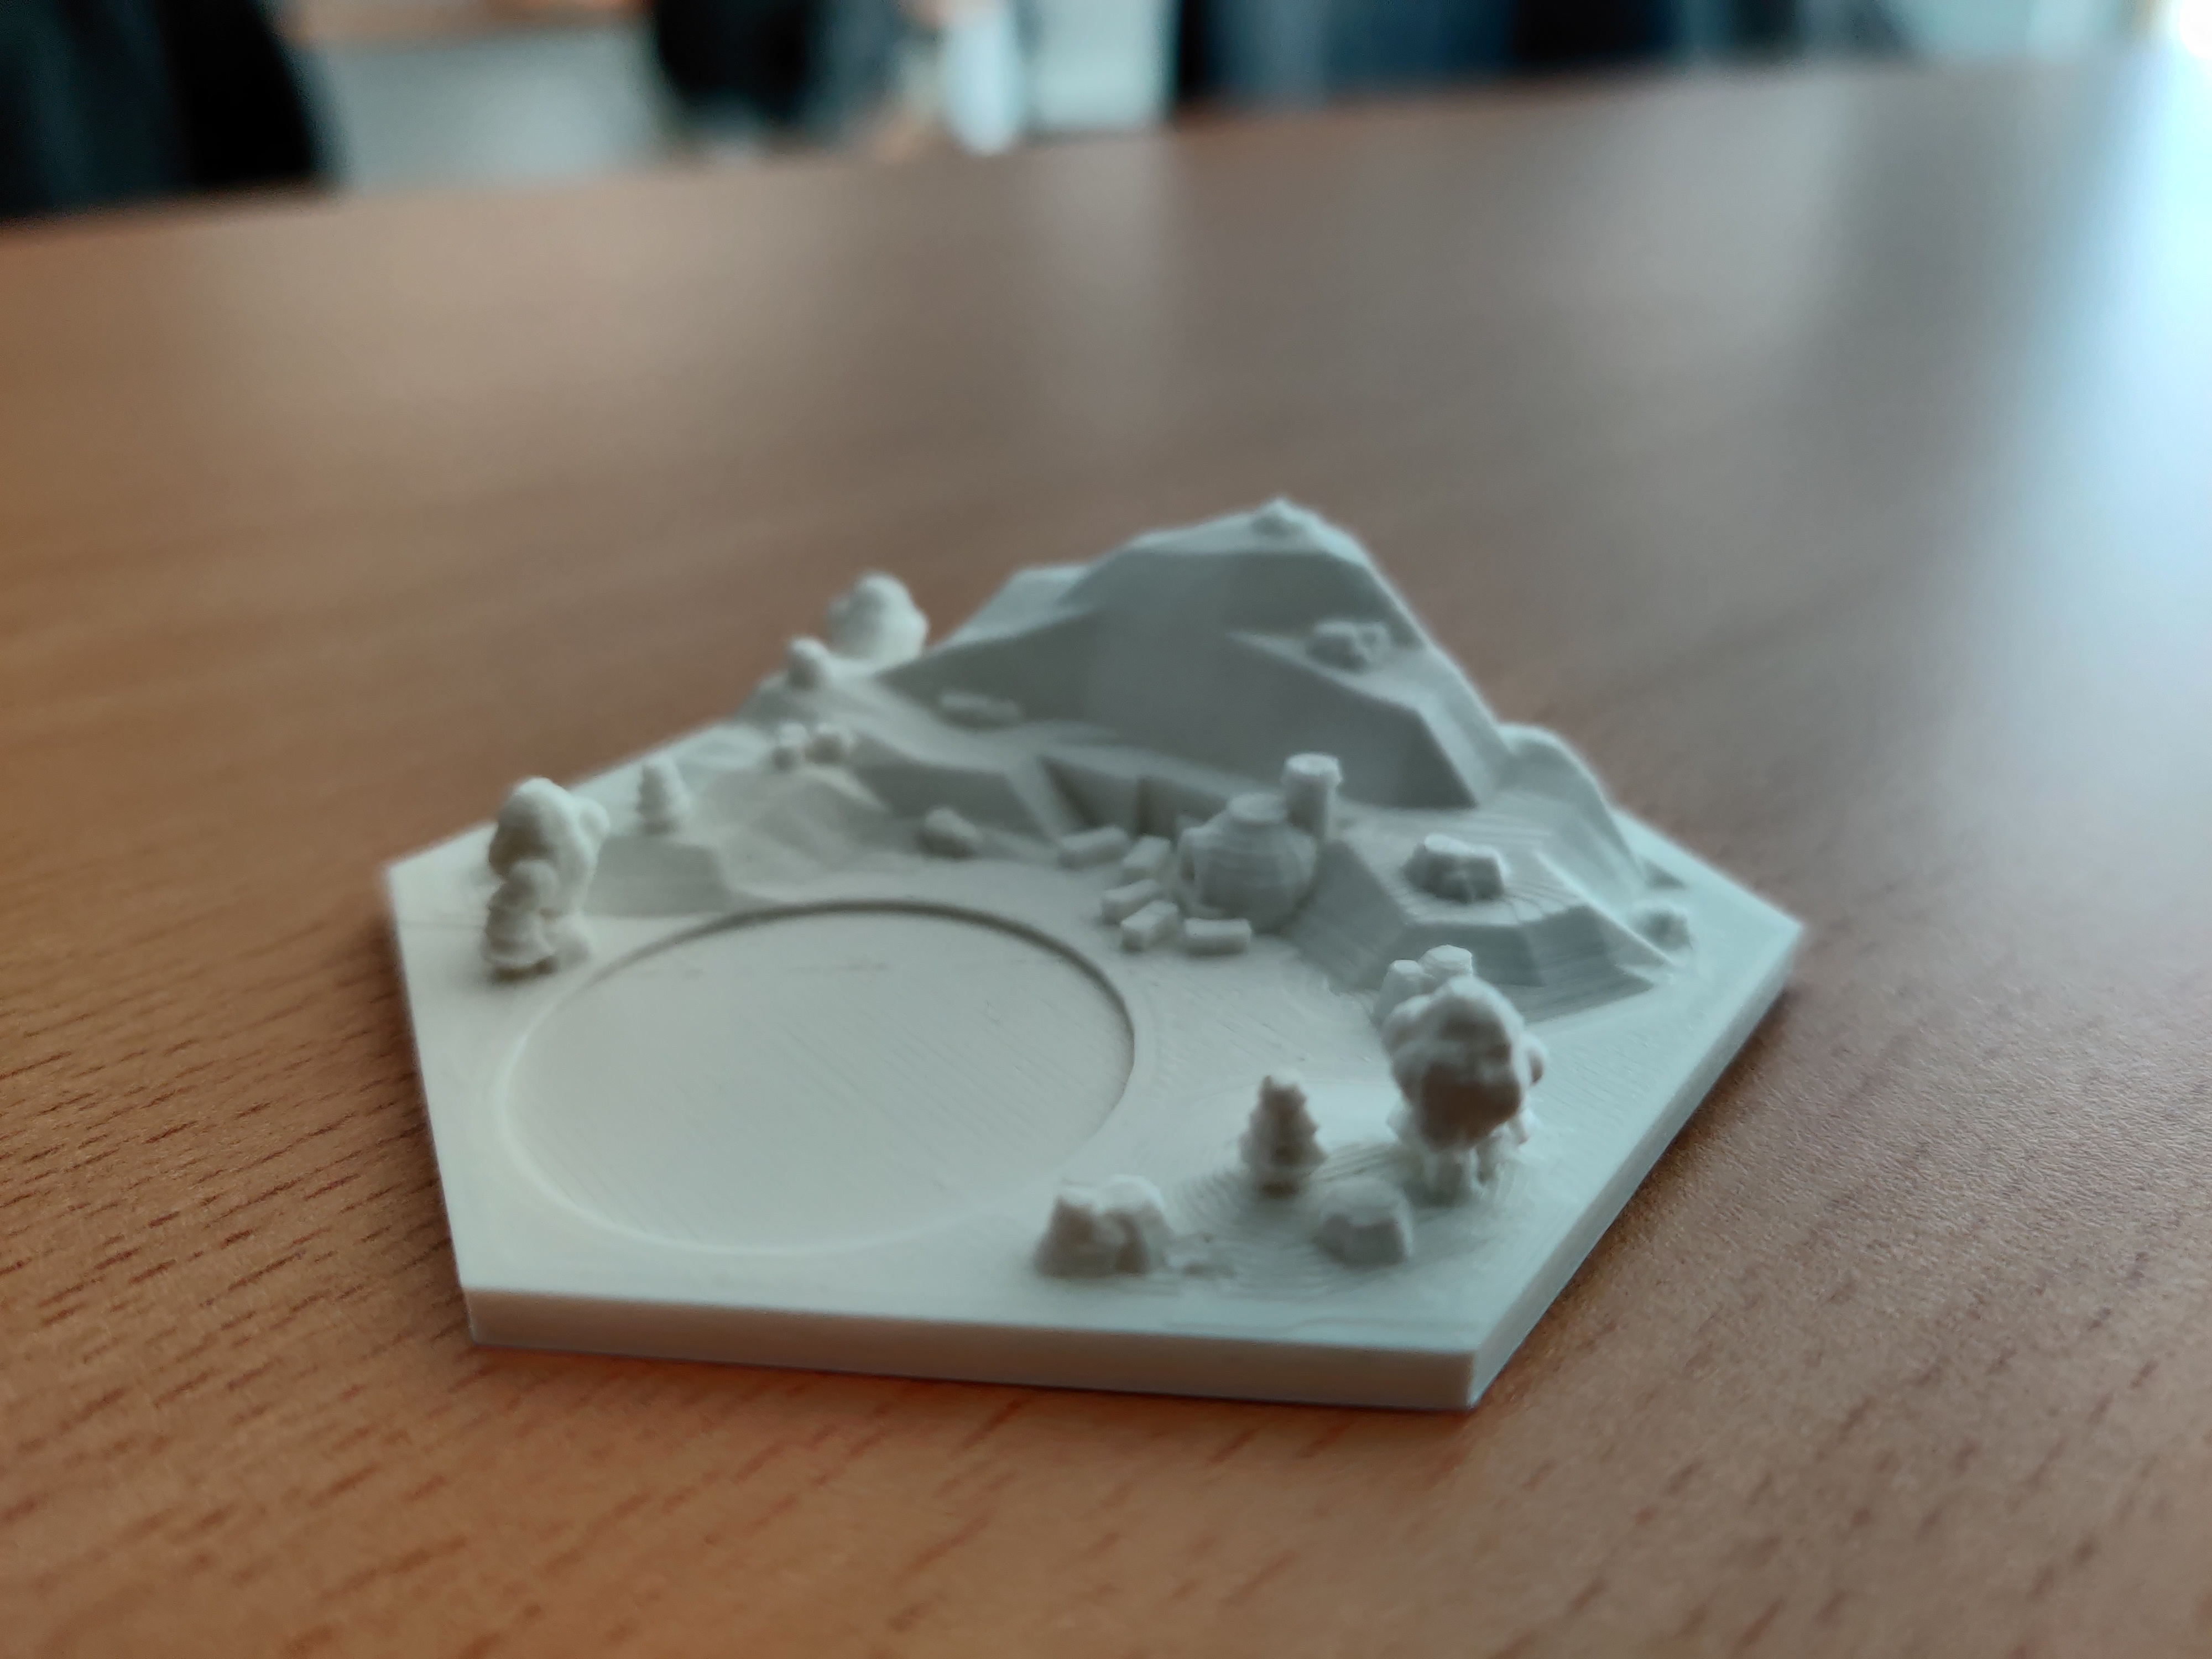
\includegraphics[width=\linewidth]{pictures/3d_test.jpg}
    \end{minipage}
    \hfill
    \begin{minipage}{.48\linewidth}
        \centering
        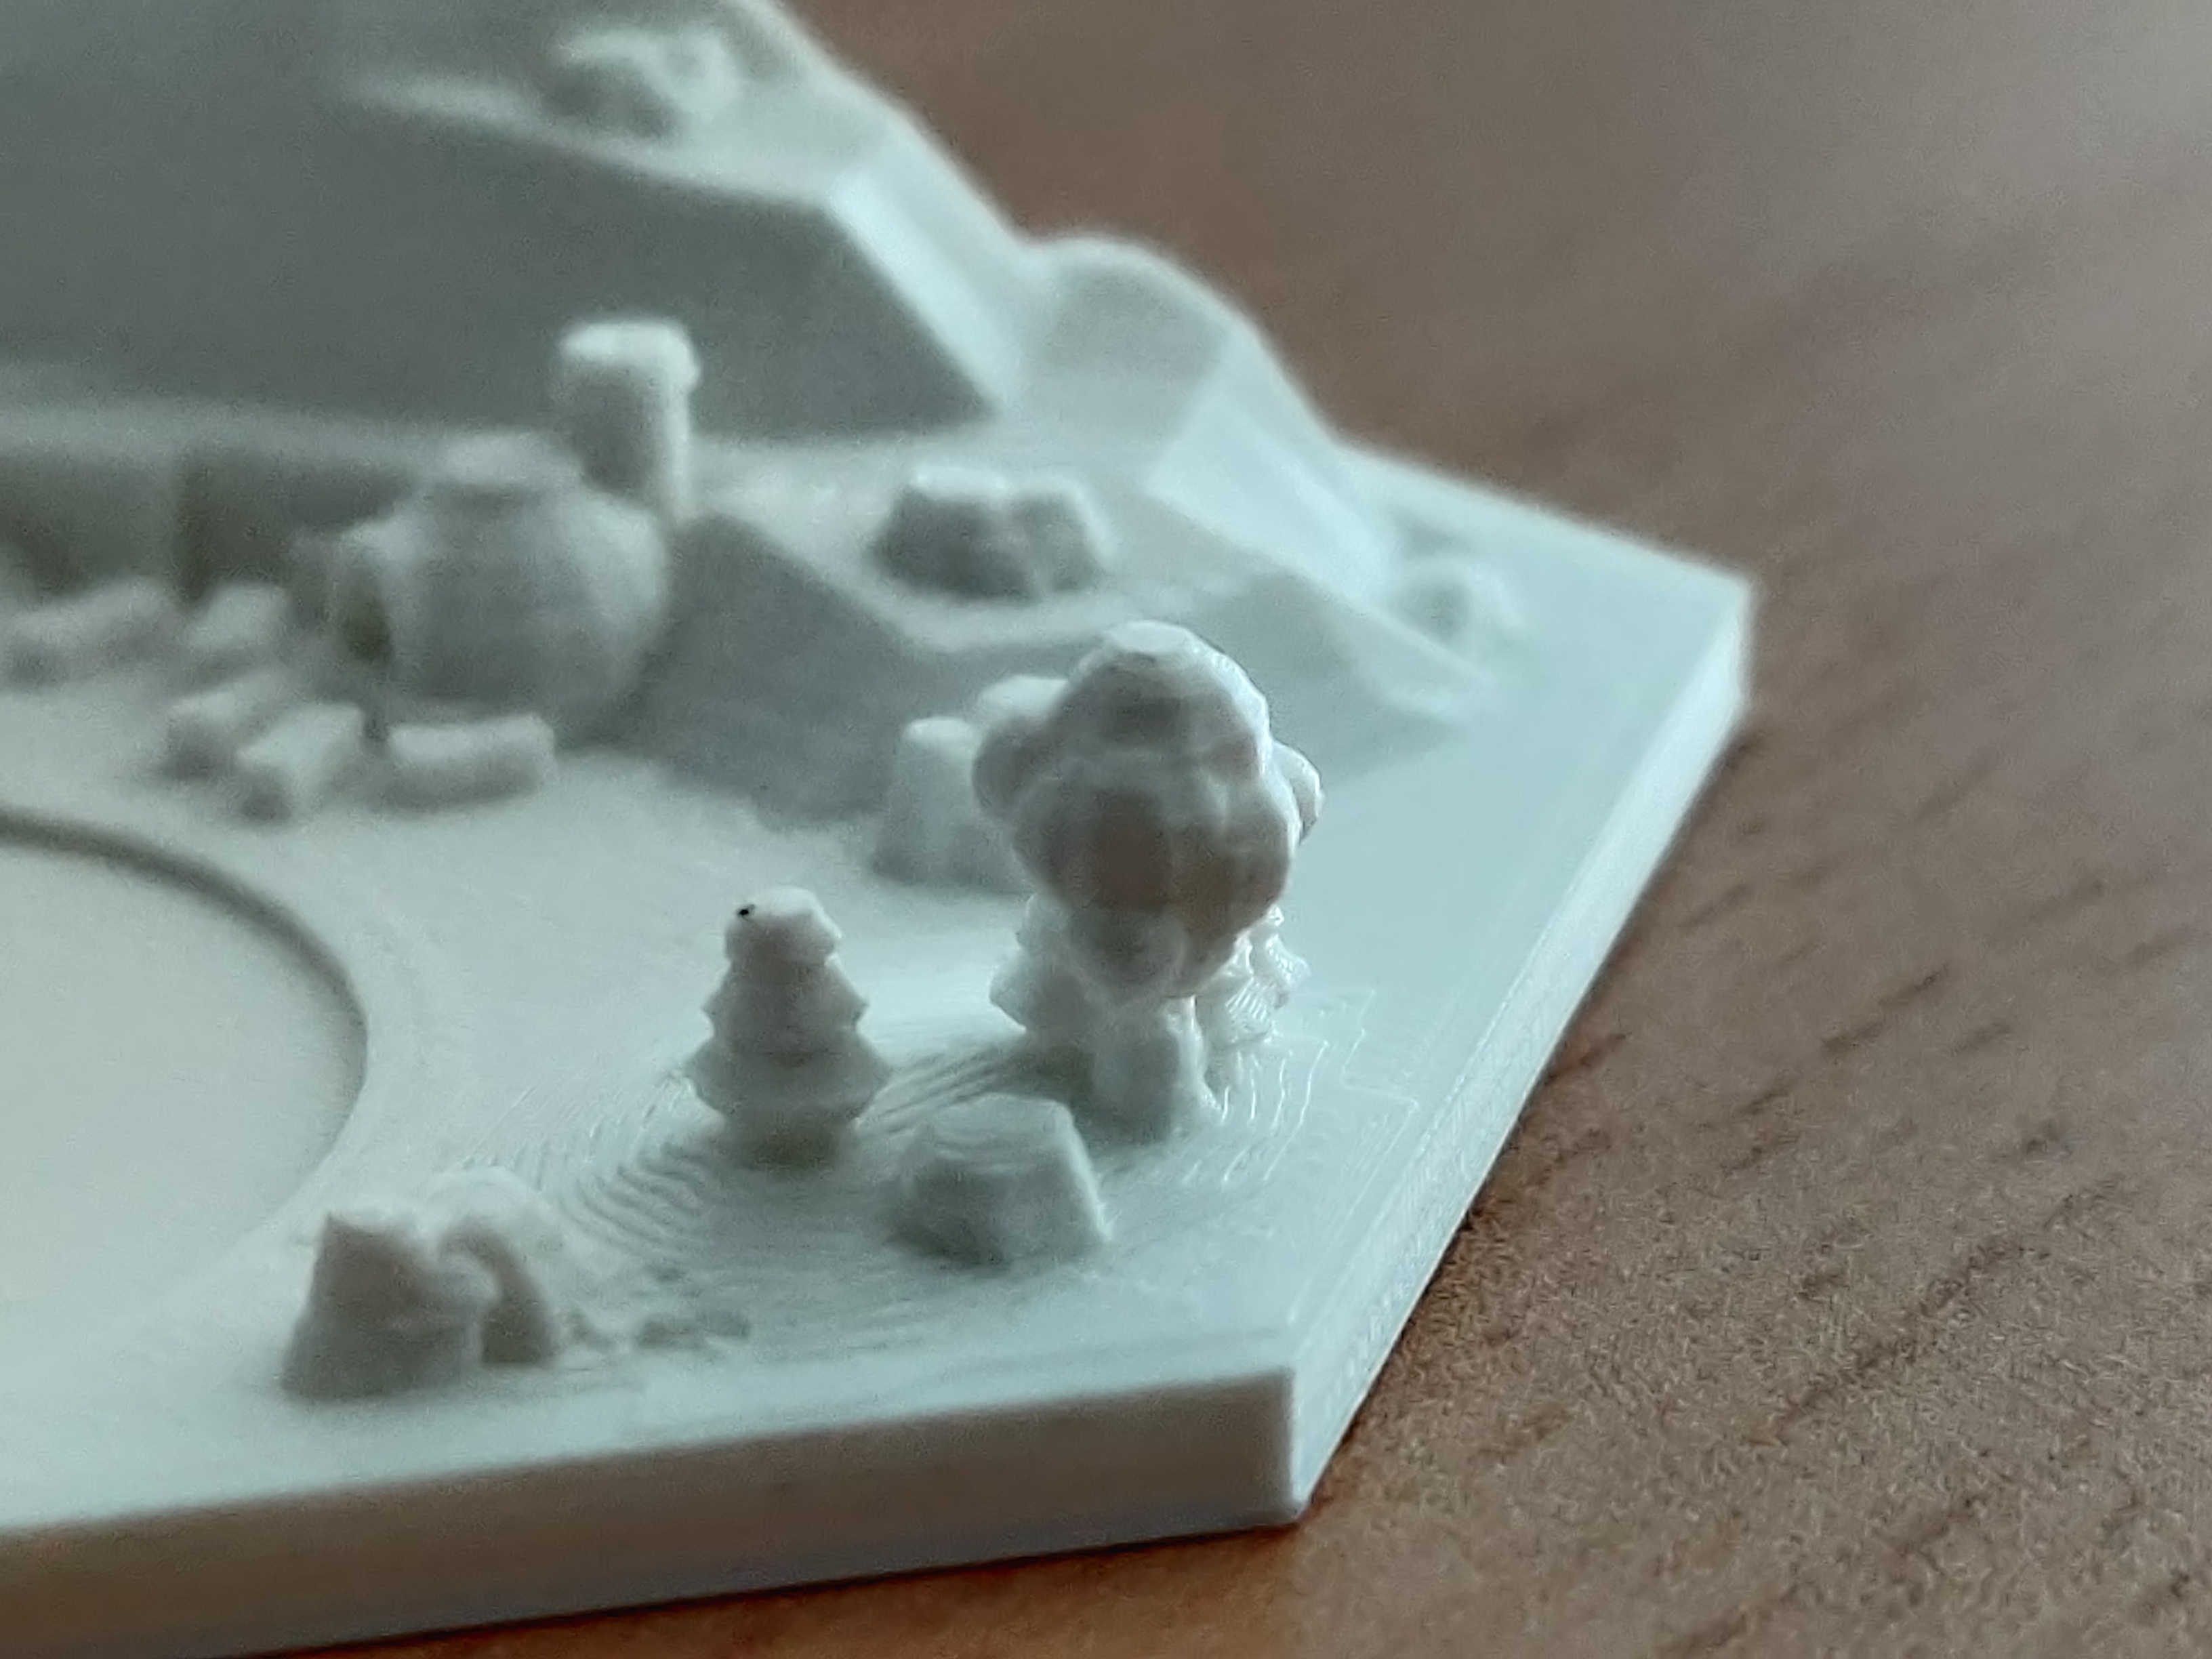
\includegraphics[width=\linewidth]{pictures/3d_test_detail.jpg}
    \end{minipage}
    \caption{Figura de prueba impresa en 3D.}
    \label{fig:test_prints}
\end{figure}

\begin{figure}[H]
    \begin{minipage}{.48\linewidth}
        \centering
        \includegraphics[width=\linewidth]{pictures/clogged_extruders.jpg}
    \end{minipage}
    \hfill
    \begin{minipage}{.48\linewidth}
        \centering
        \includegraphics[width=\linewidth]{pictures/extruded_ball.jpg}
    \end{minipage}
    \caption{Extrusores bloqueados y parcialmente dañados por una bola de plástico.}
    \label{fig:3d_extruder_fail}
\end{figure}

A partir de esta semana y hasta el momento de la entrega de este documento, el equipo de desarrollo se ha centrado en trabajar de manera paralela en el código del los dos sistemas, imprimir y refinar las distintas piezas del brazo y escribir apartados de la memoria.

Cabe destacar que el hecho de que se haya empleado tanto tiempo en estas labores durante la etapa final del proyecto es principalmente por la multitud de problemas que han ido apareciendo a medida que este ha ido avanzando, entre ellas se pueden nombrar:

\begin{itemize}
    \item Problemas con el material hidrosoluble. Este absorbe humedad del ambiente y se deteriora con el tiempo.
    \item Editar todas las piezas para adaptarlas a las métricas de los tornillos. El equipo de desarrollo llegó a la conclusión de que todas las piezas del brazo debían de ser editadas para adaptar sus medidas a los tornillo, ejes y rodamientos ya existentes.
    \item Varios problemas con la placa de control: desde el primer momento se produjeron múltiples problemas con la placa, pero empeoraron con el paso del tiempo. Los módulos de la placa de control dejaron de funcionar hasta el punto en el que la placa mostraba un funcionamiento anómalo e impredecible.
    \item El \ac{SW} de \ac{S1} tuvo que ser adaptado a
    los problemas que iban apareciendo en relación con la interconexión de la interfaz de usuario y con la lógica, esta a su vez con \ac{S2}.
\end{itemize}

Sabiendo que la fecha de inicio oficial del proyecto es el 6 de febrero de 2020 y la fecha de entrega de la memoria del proyecto es el 16 de octubre de 2020, se calcula que el periodo de desarrollo de este proyecto es de 250 días.

\subsection{Contratiempos de la impresión 3D}
\subsubsection*{Semana del 1 de julio}
En el momento en que se recibió la impresora 3D, se hicieron varias pruebas de
impresión (figura \ref{fig:test_prints}) y se comenzaron a estudiar las características
de la impresora. Se vio entonces el sistema de doble extrusor que utilizaba para
generar el material de impresión junto con el material de soporte soluble (\ac{PVA}).

\begin{figure}[H]
    \centering
    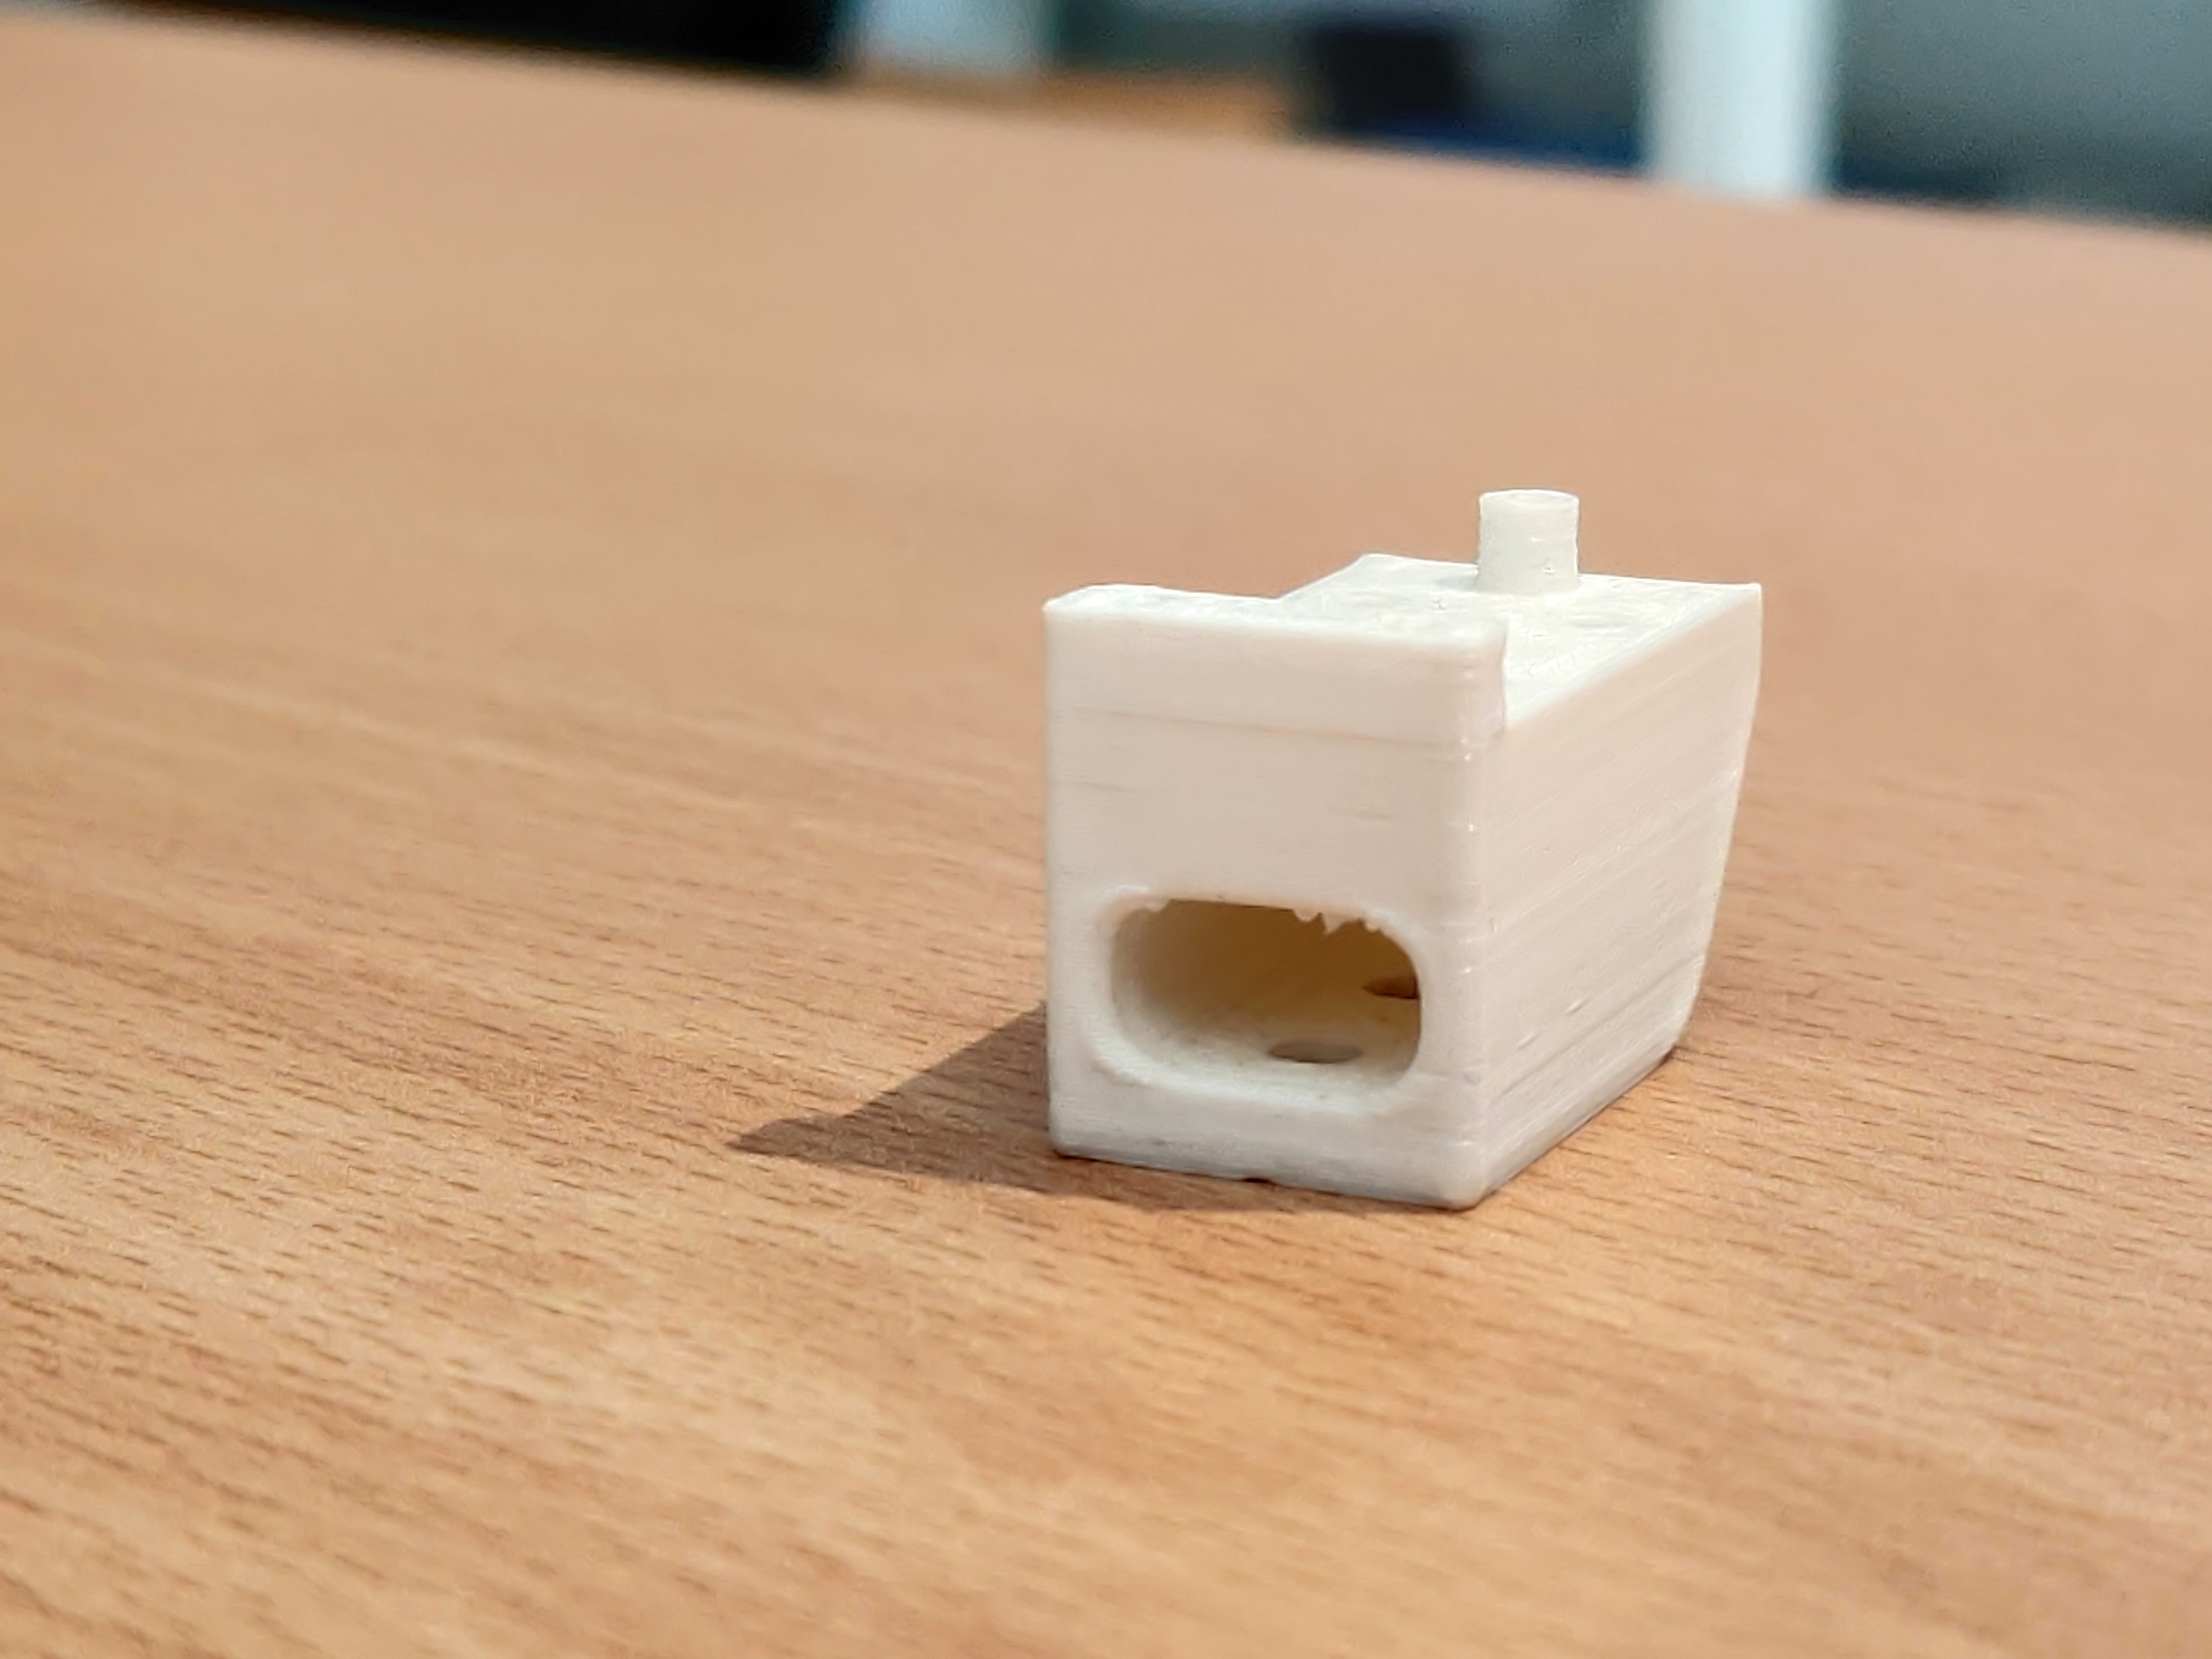
\includegraphics[width=.7\linewidth]{pictures/test_piece.jpg}
    \caption*{Pieza de prueba componente actual del \pArm{}.}
\end{figure}

Sin embargo, cuando se realizaron impresiones utilizando dicho material de soporte,
se vio que la calidad del mismo o bien no era la mejor o no bien se correspondía con
cómo debería quedar, según la web de Ultimaker (figura \ref{fig:oof_comparisson}):

\begin{figure}[H]
    \centering
    \begin{minipage}{.60\linewidth}
        \centering
        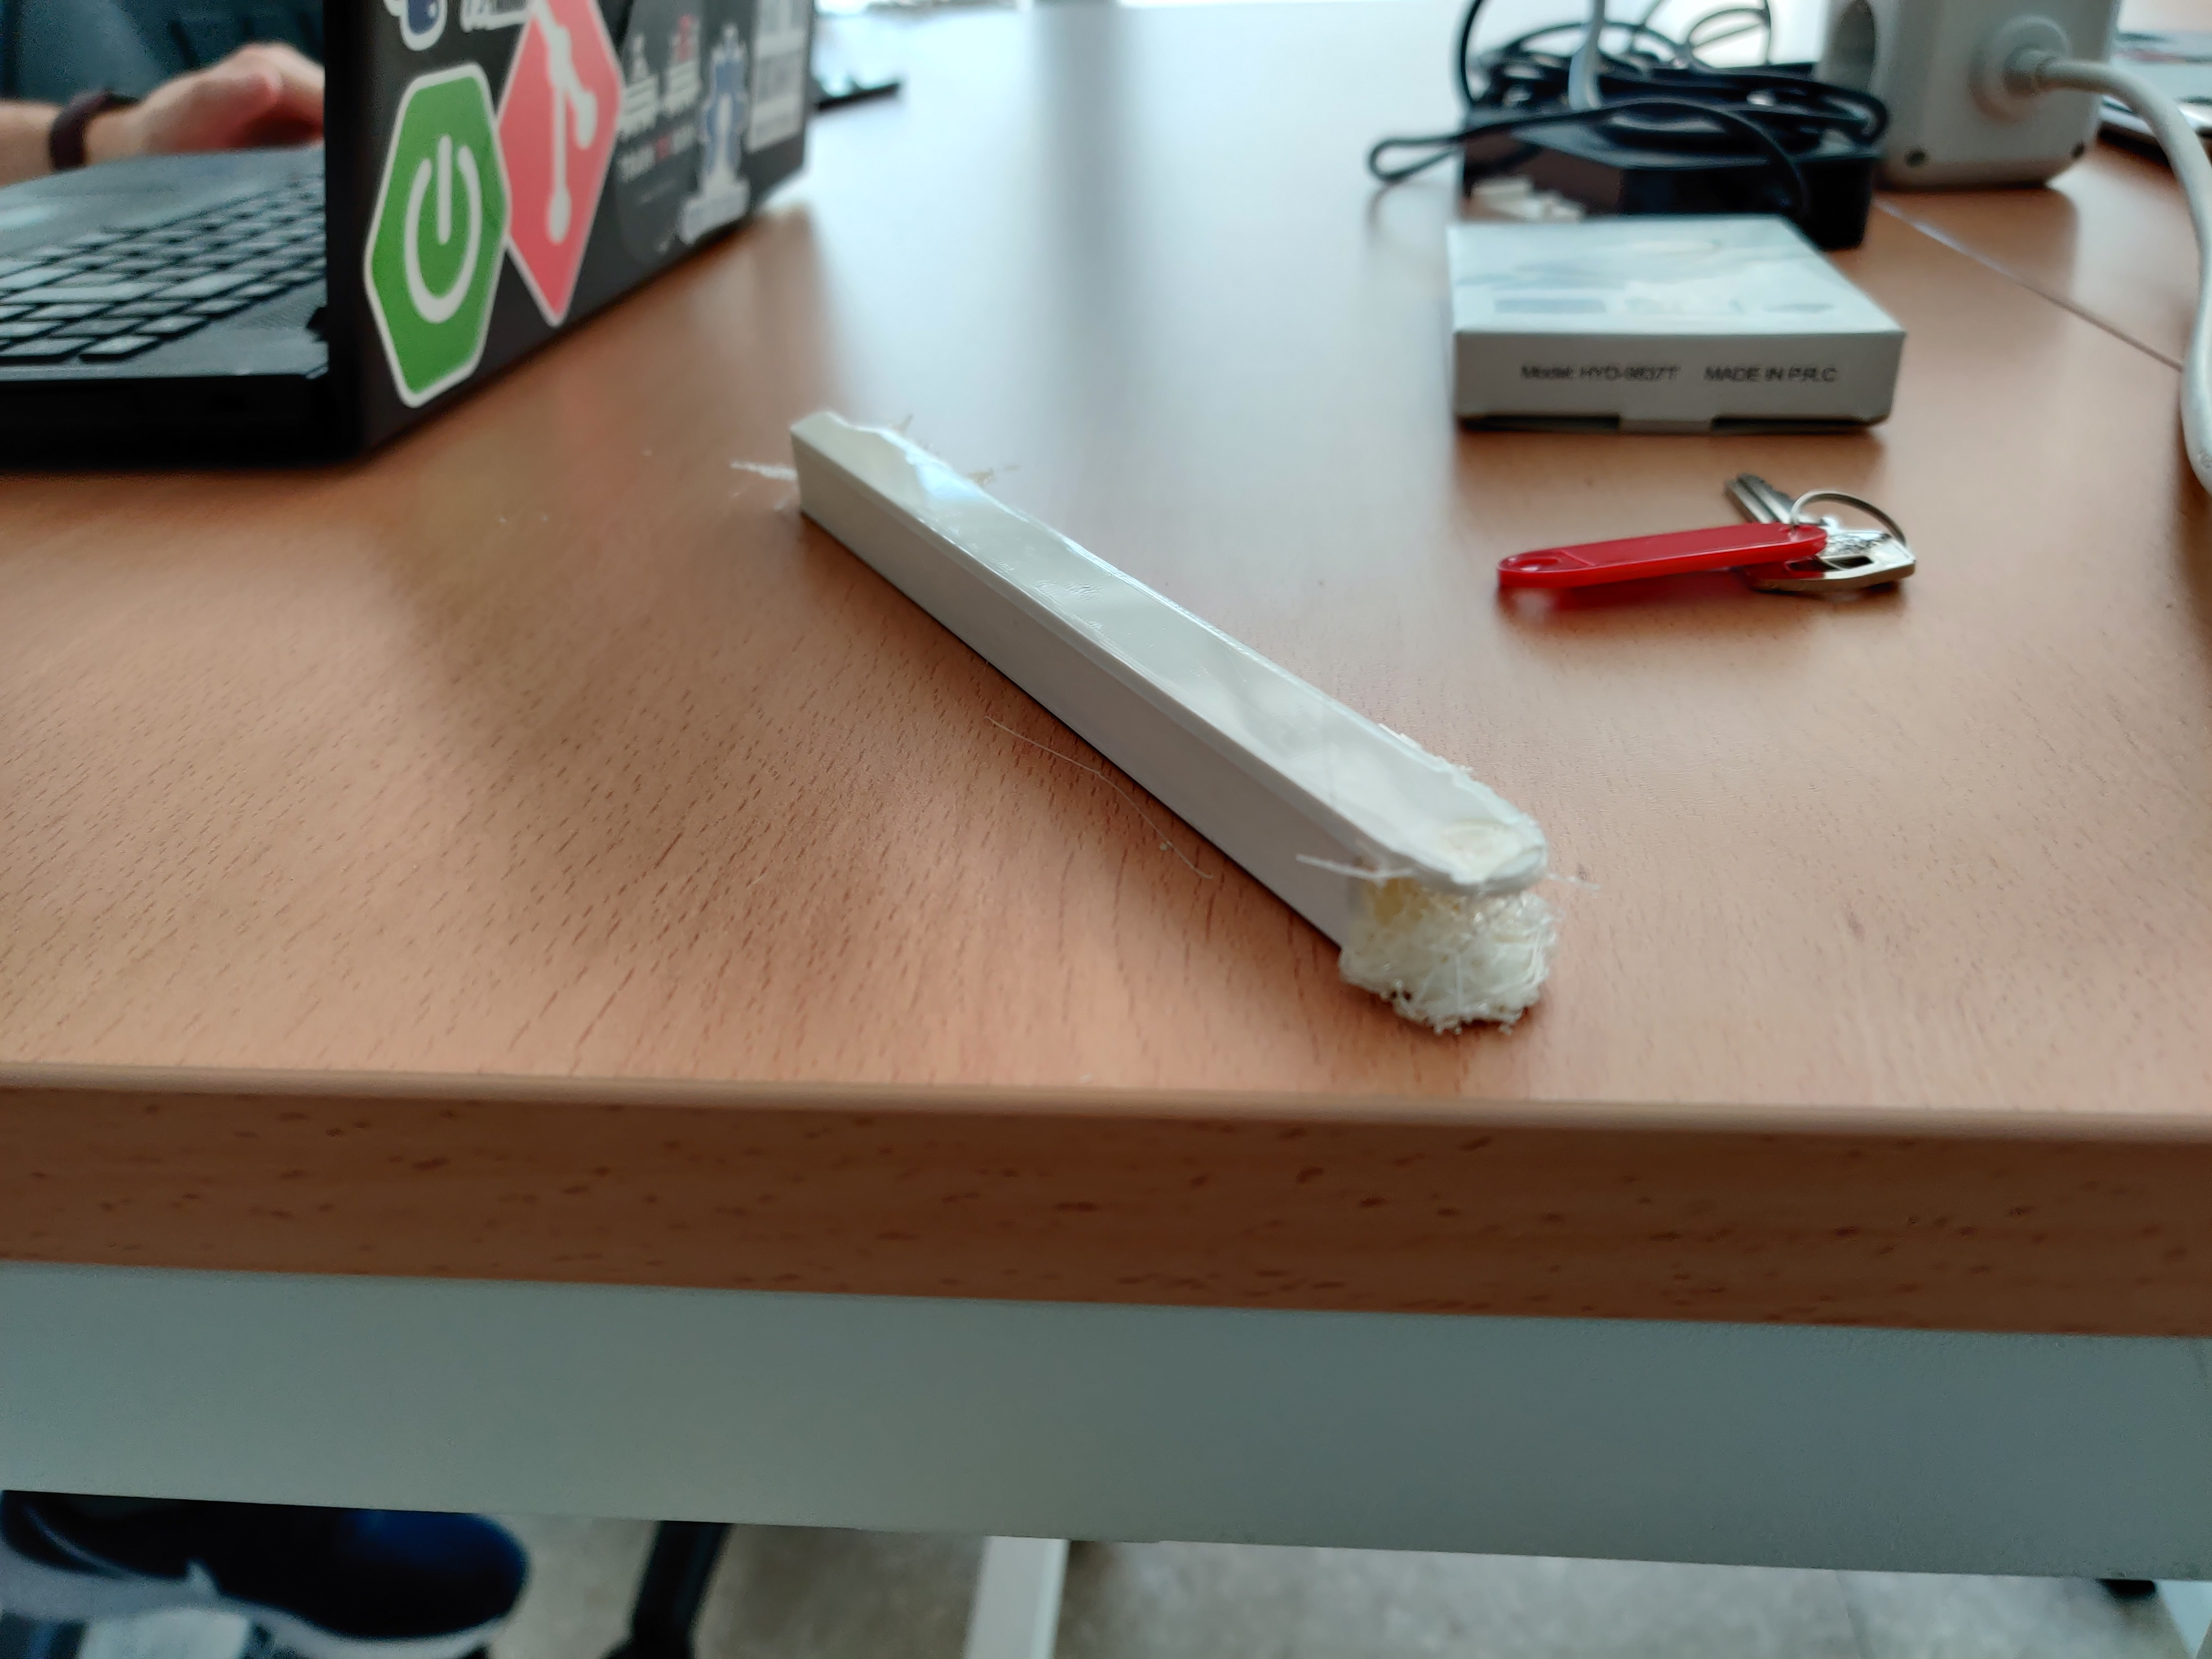
\includegraphics[width=\linewidth]{pictures/arm_oof_pva.jpg}
        \caption{Una figura de prueba que necesita \ac{PVA}.}
    \end{minipage}
    \hfill
    \begin{minipage}{.38\linewidth}
        \centering
        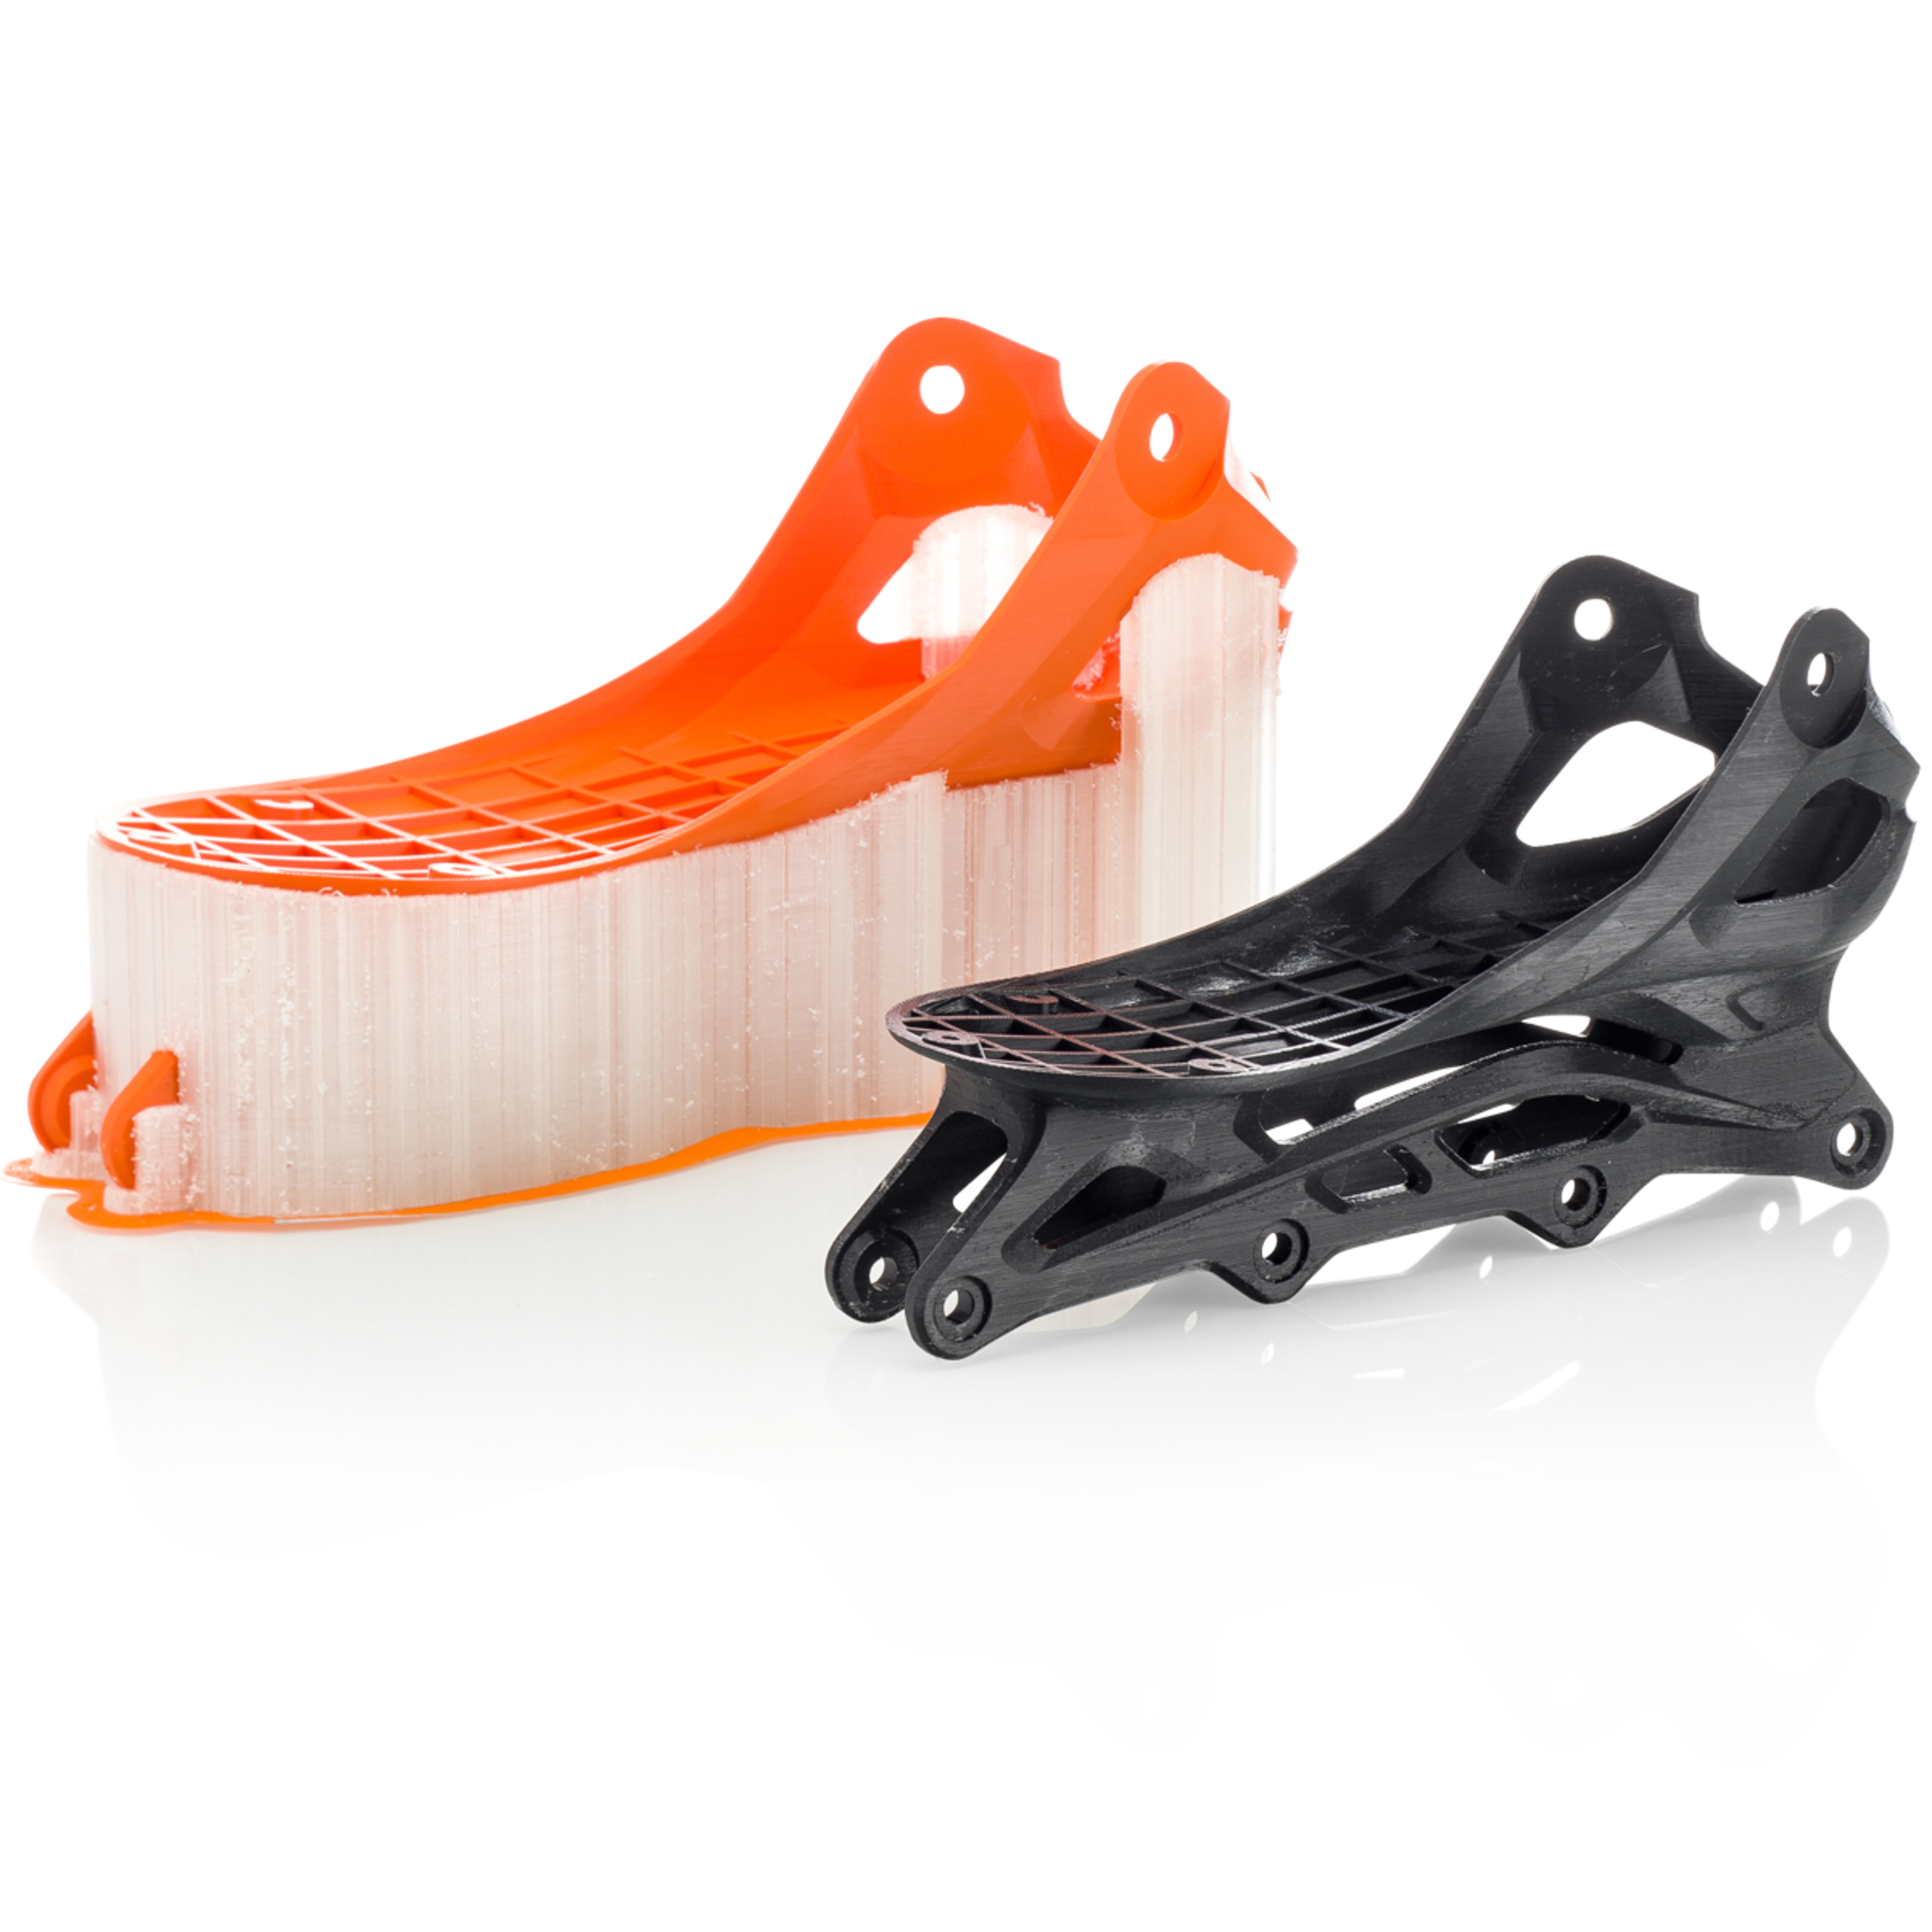
\includegraphics[width=\linewidth]{pictures/pva_support_ok.png}
        \caption{Cómo debería quedar una impresión con \ac{PVA} según Ultimaker \cite{MaterialUltimakerPVA}.}
    \end{minipage}
    \caption{Comparación de la pieza de prueba con \ac{PVA} frente a cómo deberían quedar según la web de Ultimaker.}
    \label{fig:oof_comparisson}
\end{figure}

\subsubsection*{Semana del 6 de julio}
Después de hacer múltiples pruebas con el material de soporte se observó que salían granos
color negro en lugar de un hilo de plástico, por lo que se dedujo que el material de
soporte no estaba en buen estado o que el extrusor estaba dañado. Ante esa situación,
se desmontó el \textit{nozzle} y se comprobó que en efecto estaba completamente lleno
de \ac{PVA} seco y podrido (figura \ref{fig:nozzle_oof}):

\begin{figure}[H]
    \centering
    \begin{minipage}{.49\linewidth}
        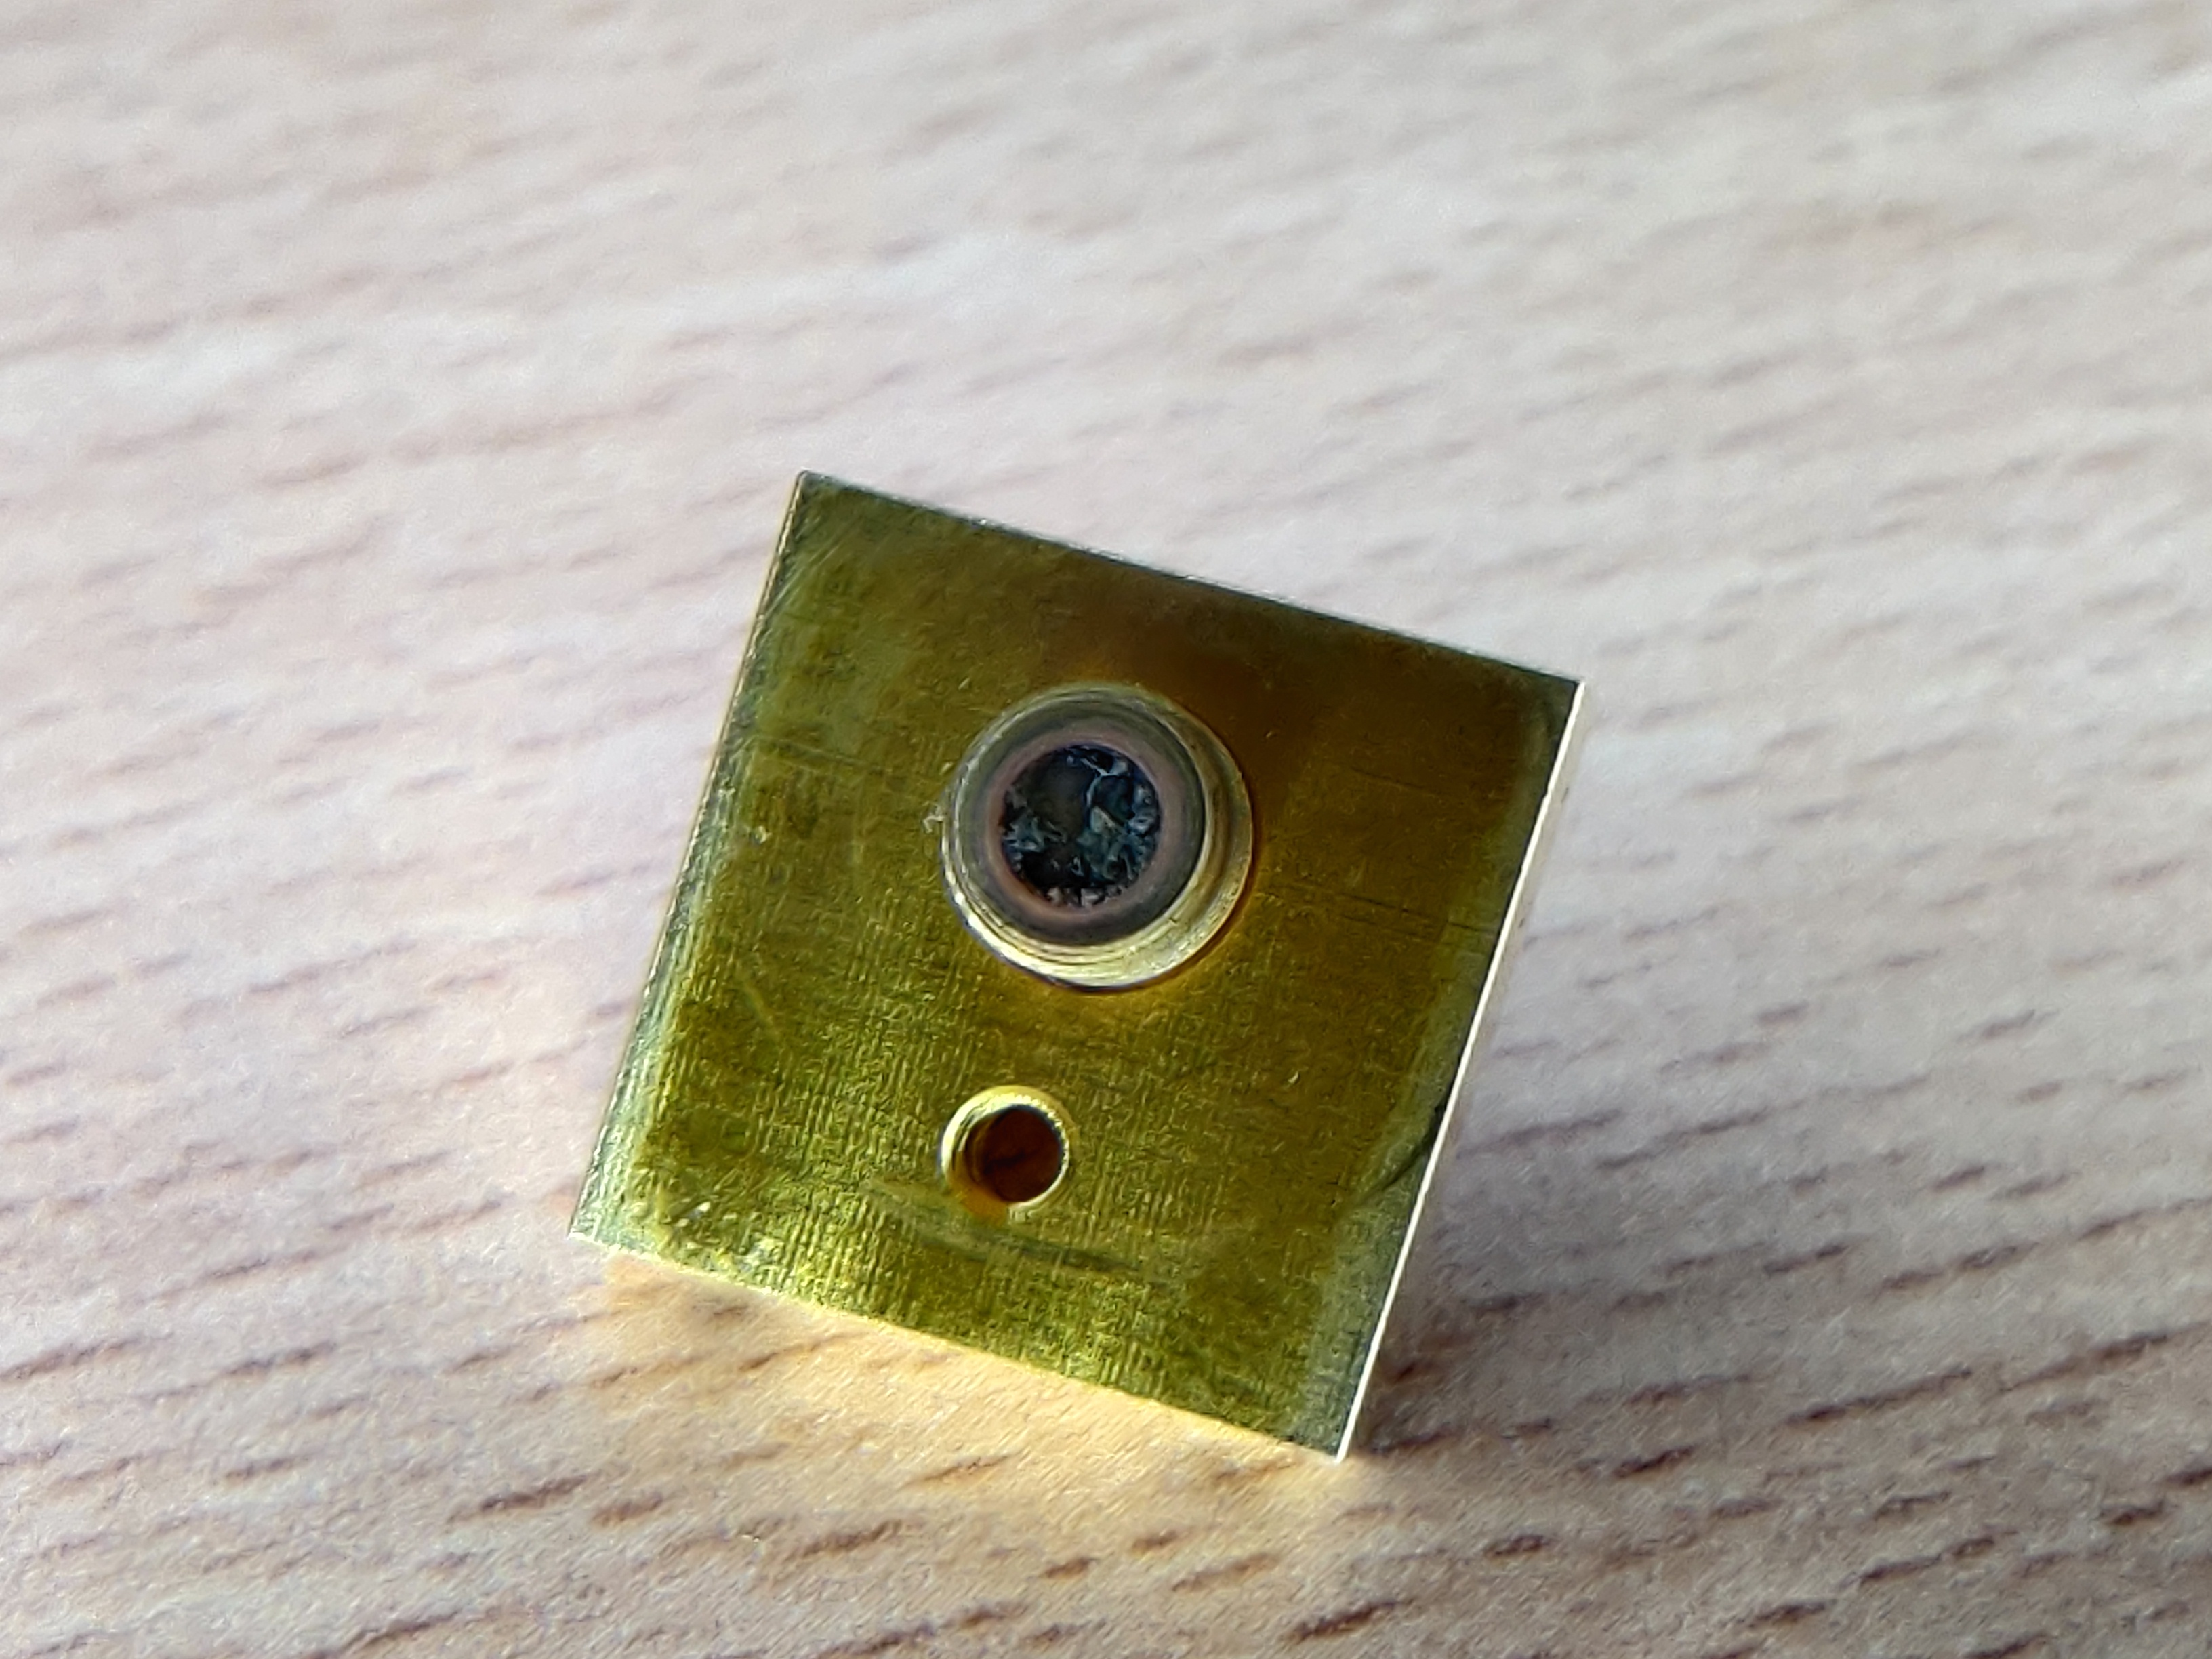
\includegraphics[width=\linewidth]{pictures/clogged_nozzle.jpg}
    \end{minipage}
    \hfill
    \begin{minipage}{.49\linewidth}
        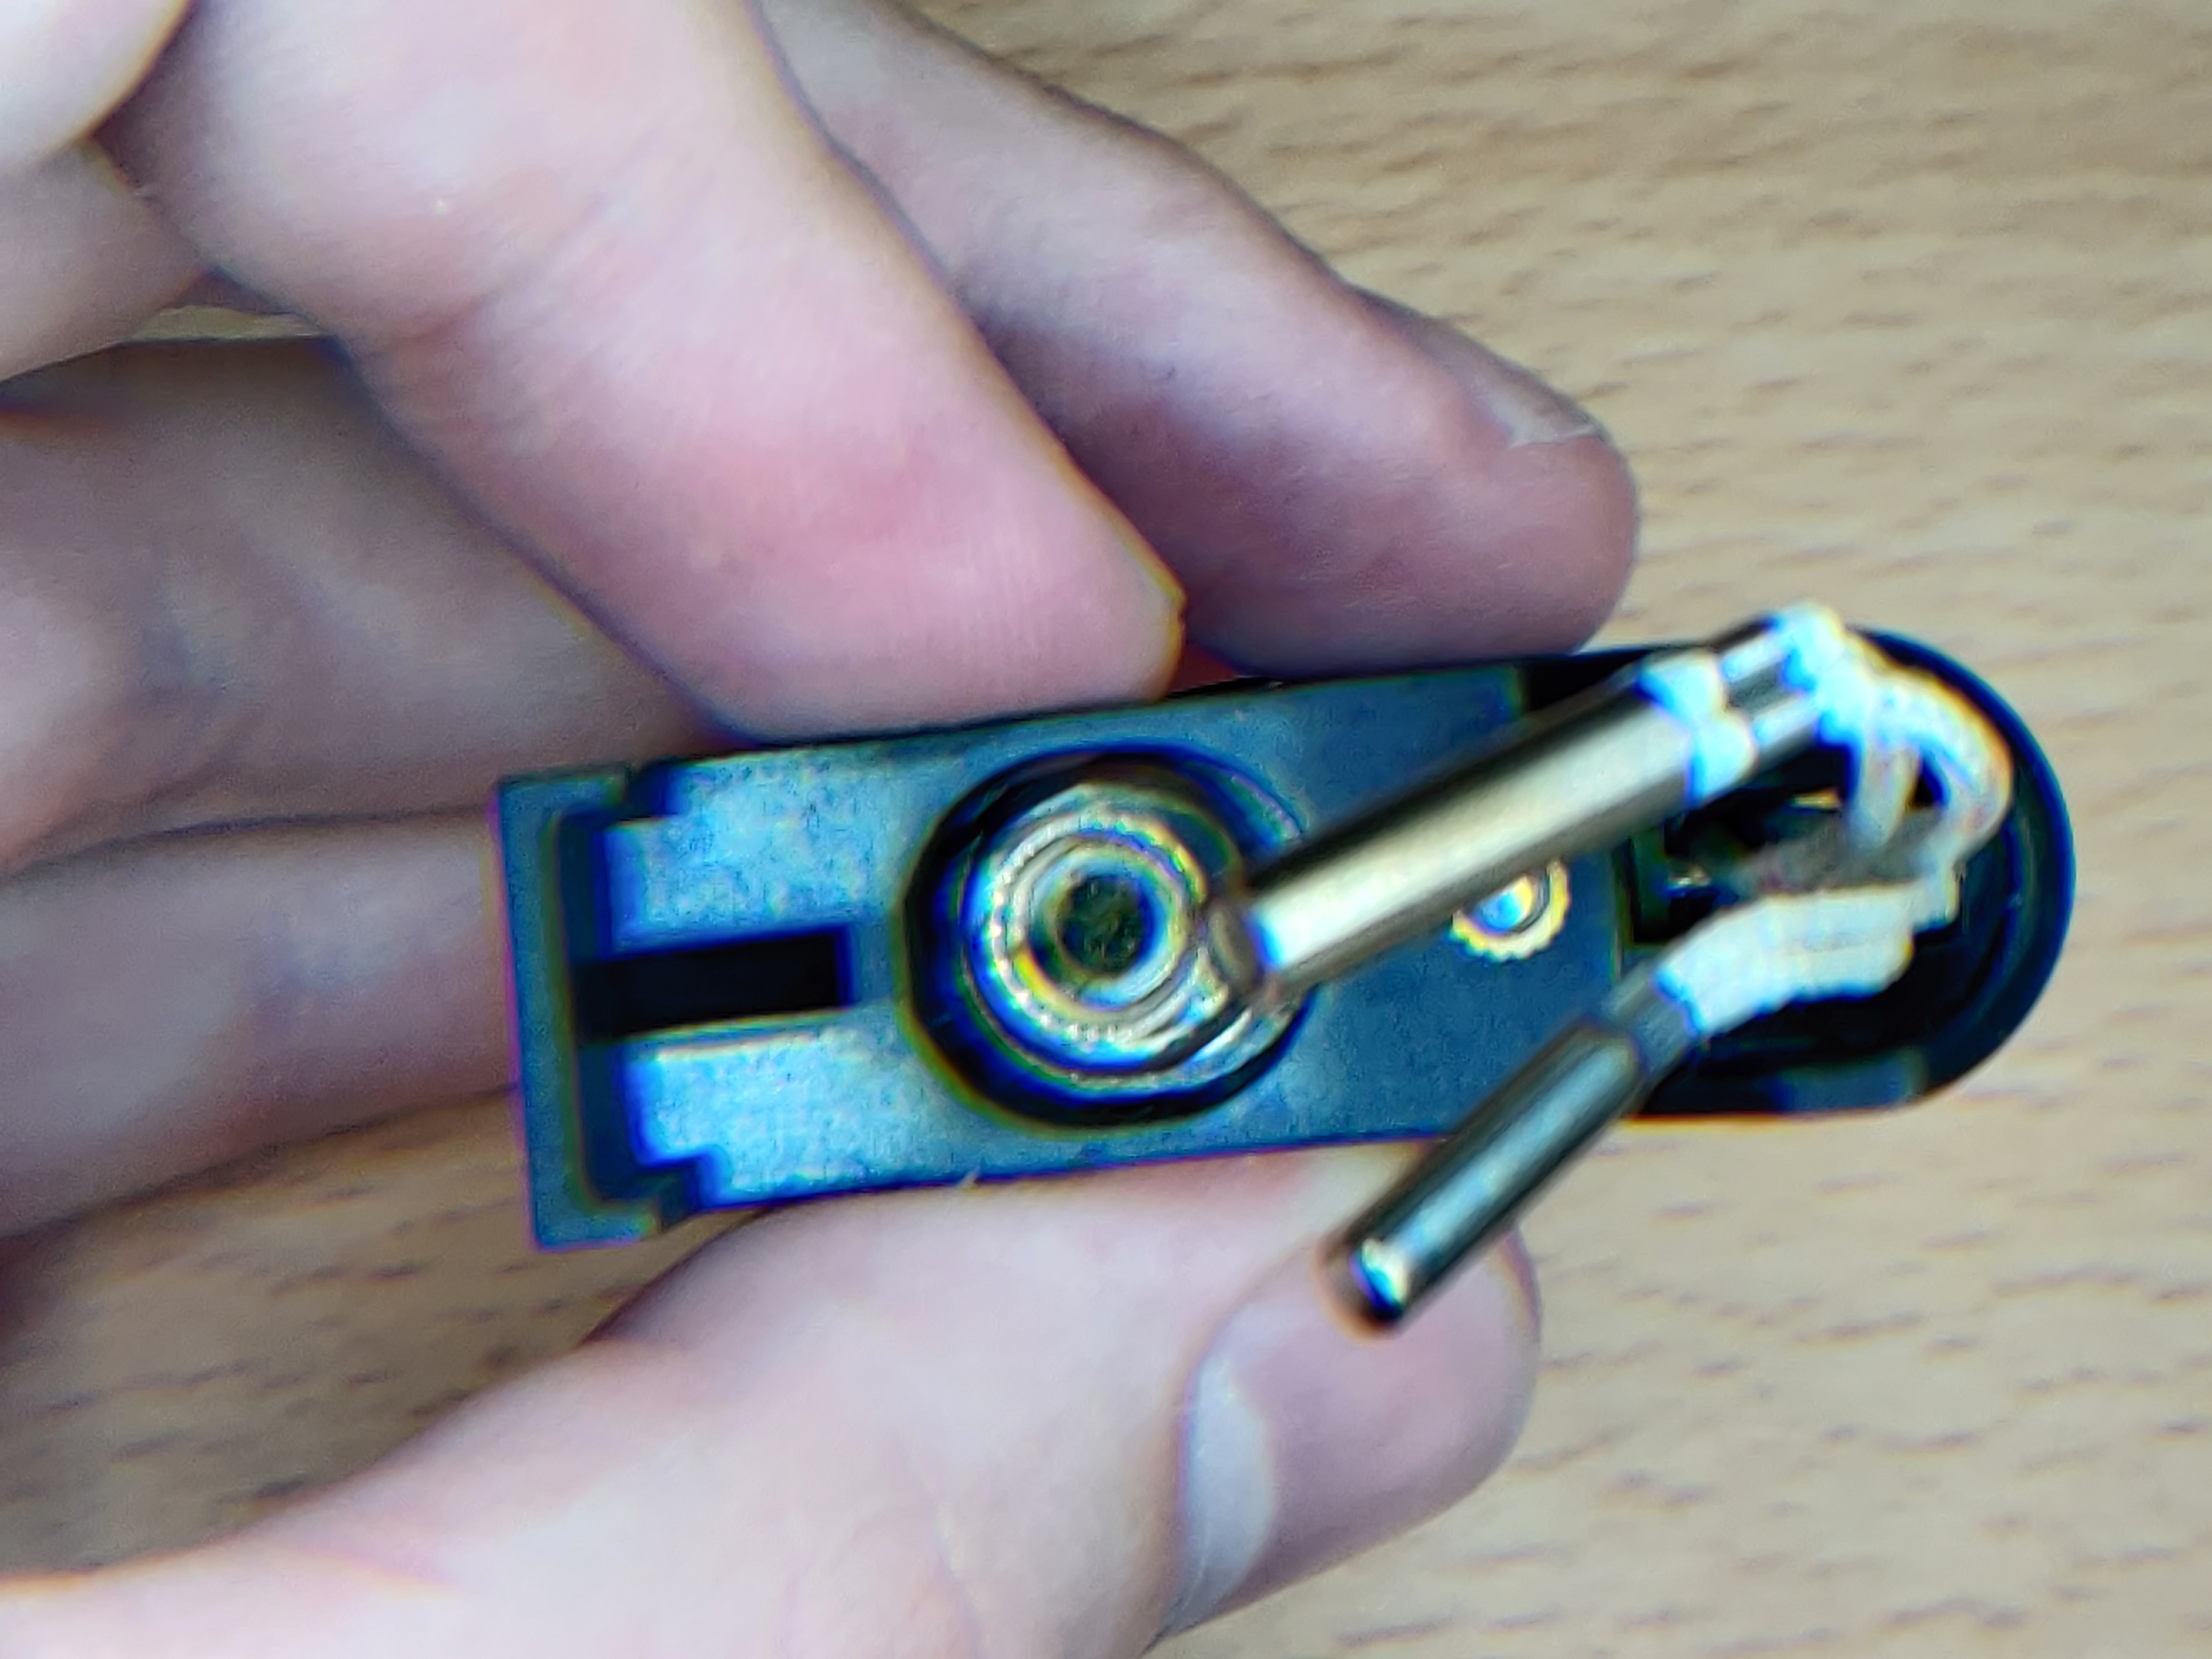
\includegraphics[width=\linewidth]{pictures/nozzle_oof_2.jpg}
    \end{minipage}
    \caption{\textit{Nozzle} completamente obstruído con \ac{PVA}.}        
    \label{fig:nozzle_oof}
\end{figure}

Como estaba lleno de \ac{PVA}, se optó por dejar el \textit{nozzle} en remojo para
intentar que el material de soporte se disuelva. Tras varios días, una gran parte
pudo ser quitada pero todavía quedaba bastante en su interior, que tuvo que ser
retirada manualmente.

Igualmente, tras poder utilizar nuevamente el \textit{nozzle} para generar material
de soporte, este quedó nuevamente bloqueado cuando se imprimió con él múltiples veces. Se dedujo
entonces que el material \ac{PVA} estaba dañado posiblemente por el usuario anterior. Como se
comentó en el apartado de impresión 3D, es un material que absorbe rápidamente la
humedad y que si, además, se encuentra expuesto a la luz se agrava el daño recibido.
Cuando se recibió la impresora, el material estaba completamente expuesto al ambiente
además de no estar protegido siquiera contra la luz.

\subsubsection*{Semana del 13 de julio}
Tras realizar una investigación sobre este problema, se descubrió que era algo
común a los usuarios que utilizaban \ac{PVA} como material de soporte y que se
solucionaba guardando los plásticos de impresión en una caja aislada del exterior
junto con un purificador de aire que absorbe humedad\footnote{Se puede encontrar
la caja empleada en Thingiverse: \url{https://www.thingiverse.com/thing:2756012}}.

En la figura \ref{fig:dry_box} se puede ver el resultado final:

\begin{figure}[H]
    \centering
    \begin{minipage}{.49\linewidth}
        \centering
        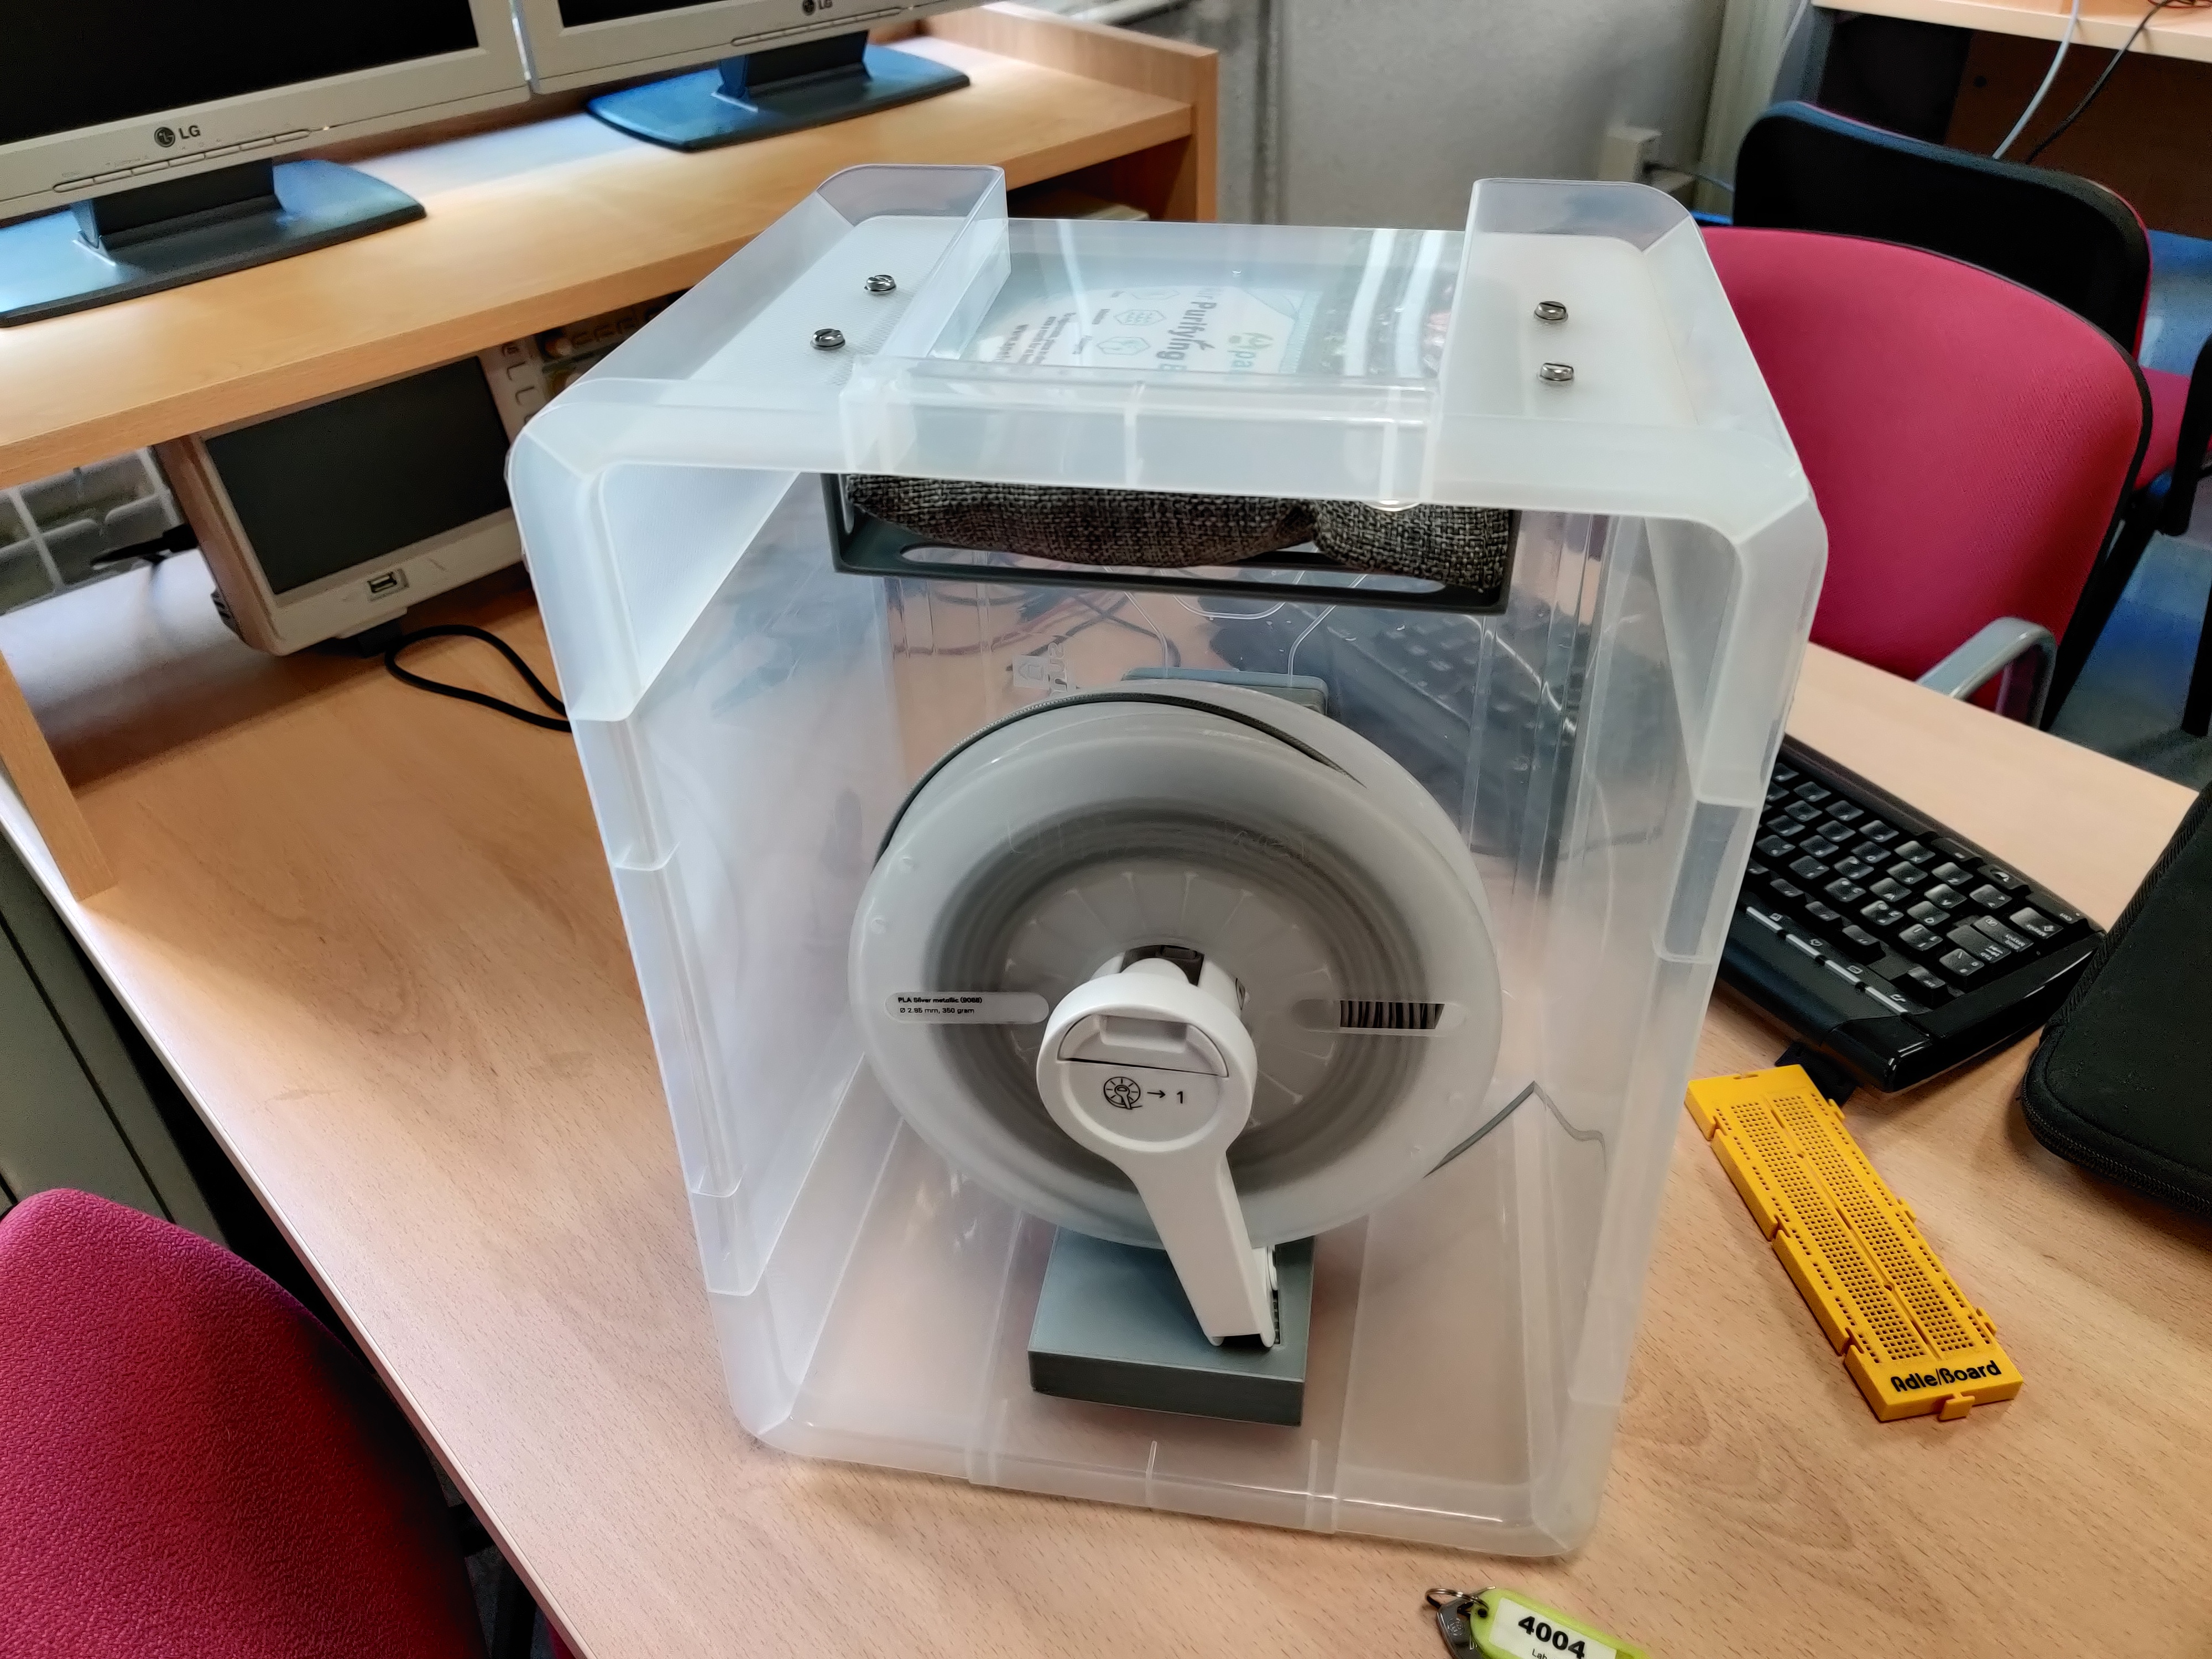
\includegraphics[width=\linewidth]{pictures/dry_box_1.jpg}
    \end{minipage}
    \hfill
    \begin{minipage}{.49\linewidth}
        \centering
        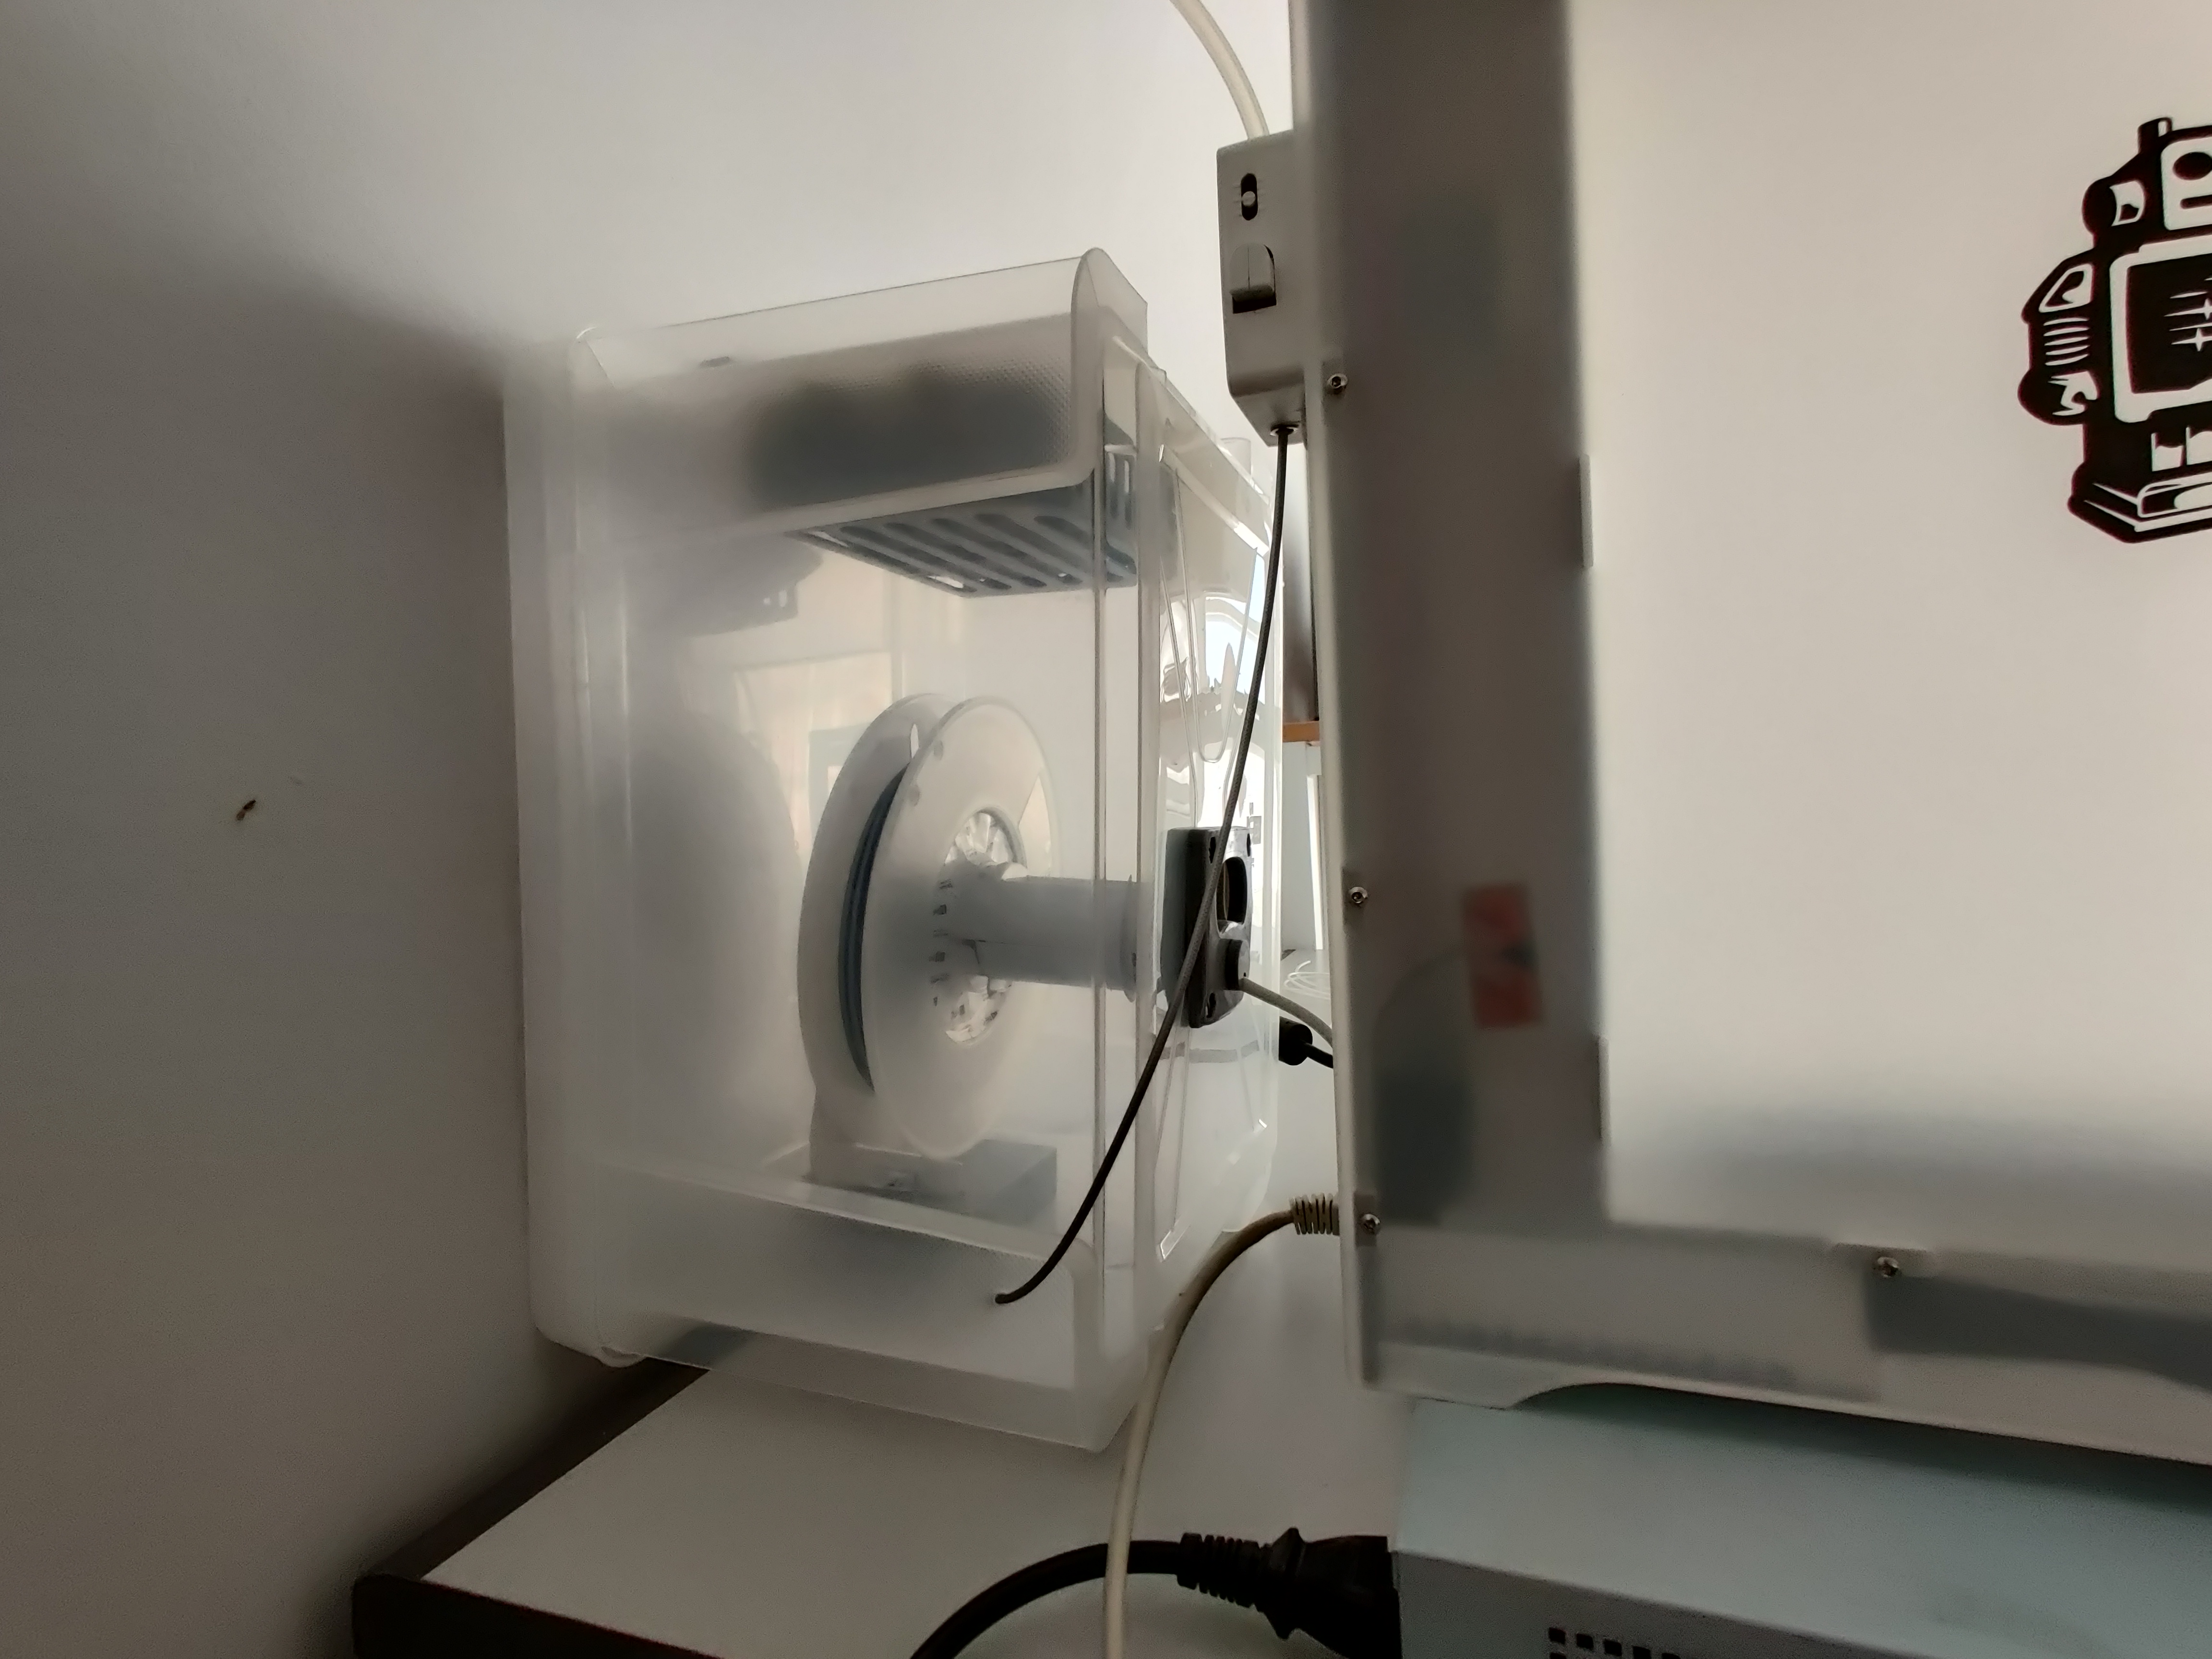
\includegraphics[width=\linewidth]{pictures/dry_box_2.jpg}
    \end{minipage}
    \caption{Caja para guardar los plásticos de impresión y mantenerlos protegidos de la humedad.}
    \label{fig:dry_box}
\end{figure}

\subsubsection*{Semana del 20 de julio}
Tras intentar aproximar el problema anterior, la impresión con \ac{PVA} seguía sin
salir como se buscaba, por lo que fue necesario comprar un nuevo hilo de dicho material.

Se empezó además a trabajar con material de impresión \ac{CPE}, pero ocurrió un nuevo
imprevisto al imprimir cuando el cabezal de impresión se chocó contra una de las piezas
que estaban siendo impresas, provocando que se generase una bola de plástico alrededor 
de los extrusores, dejándolos bastante dañados (figura \ref{fig:damaged_nozzle}).

\begin{figure}[H]
    \centering
    \begin{minipage}{.49\linewidth}
        \includegraphics[width=\linewidth]{pictures/damaged_nozzle_2.jpg}
    \end{minipage}
    \hfill
    \begin{minipage}{.49\linewidth}
        \includegraphics[width=\linewidth]{pictures/extruded_ball.jpg}
    \end{minipage}
    \hfill \\[1ex]
    \includegraphics[width=.9\linewidth]{pictures/damaged_nozzle.jpg}
    \caption{Los extrusores bloqueados y dañados tras una colisión con una pieza.}
    \label{fig:damaged_nozzle}
\end{figure}

\subsubsection*{Semana del 3 de agosto}
Se consiguieron arreglar los extrusores después de la obstrucción anterior, se pudieron
empezar a imprimir diversas piezas que requerían de soporte con \ac{PVA} de forma
exitosa, obteniendo los resultados deseados (ver figura \ref{fig:good_pieces}):

\begin{figure}[H]
    \centering
    \begin{minipage}{.49\linewidth}
        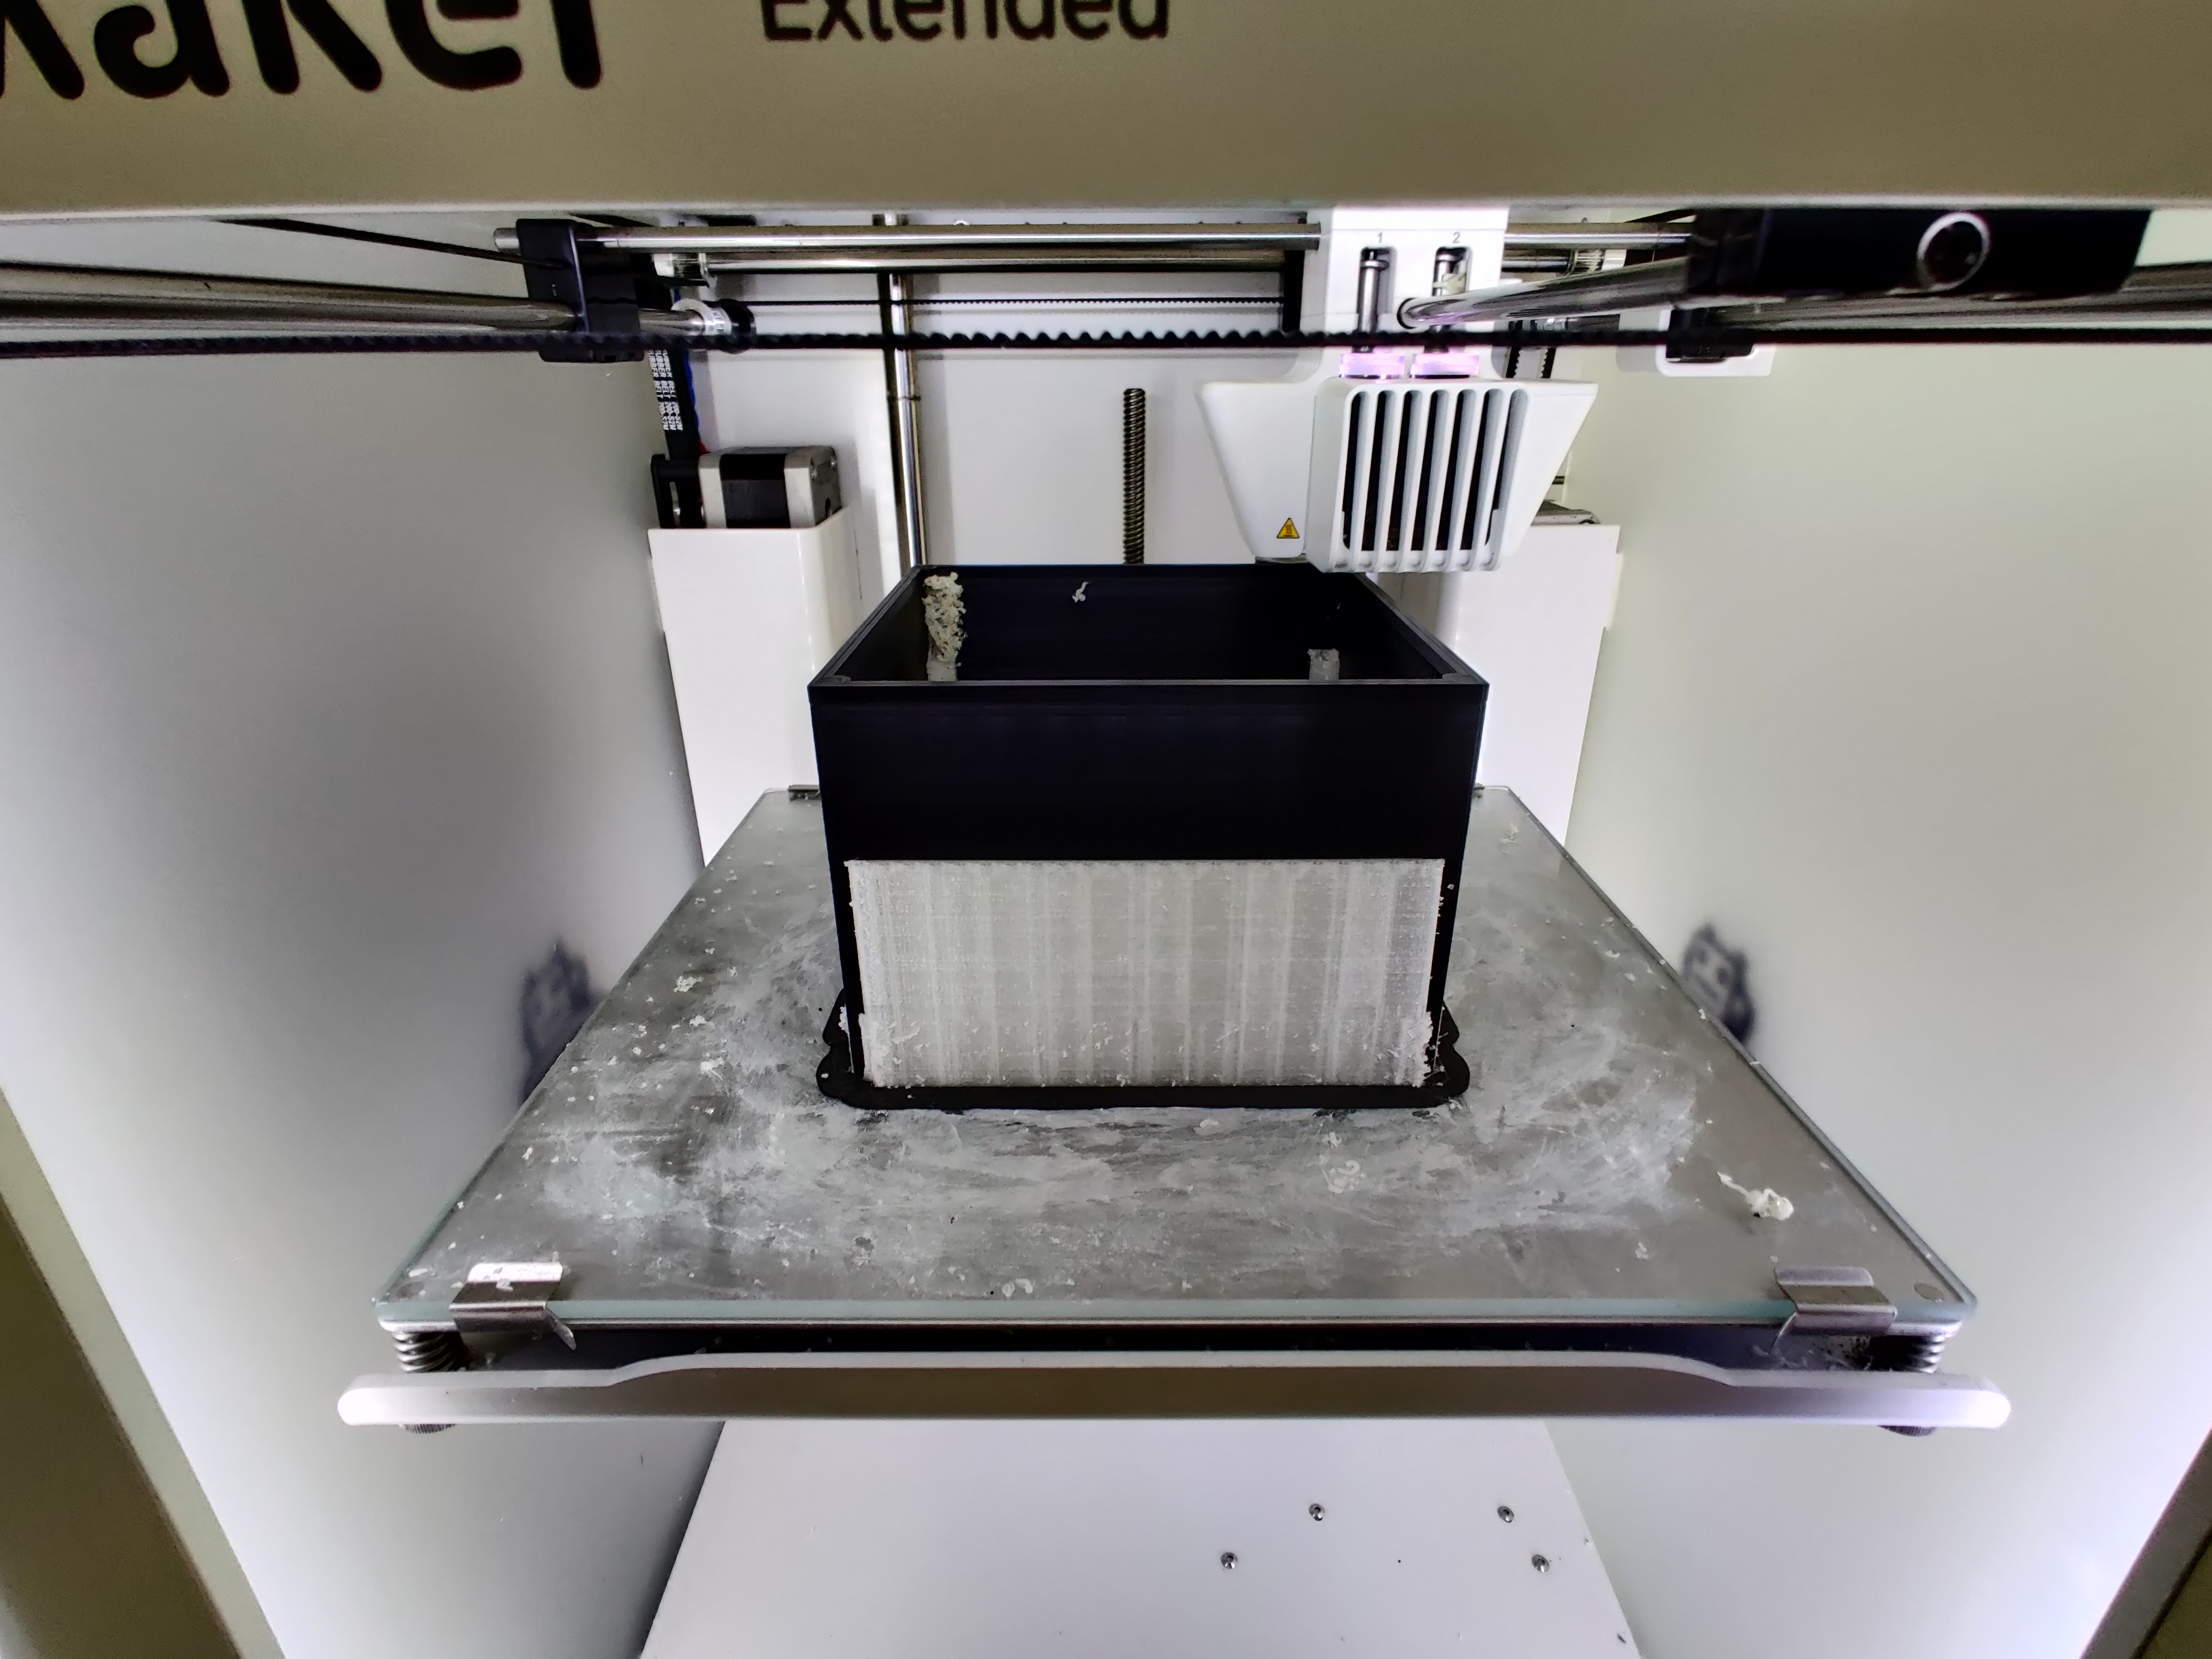
\includegraphics[width=\linewidth]{pictures/box_good.jpg}
    \end{minipage}
    \hfill
    \begin{minipage}{.49\linewidth}
        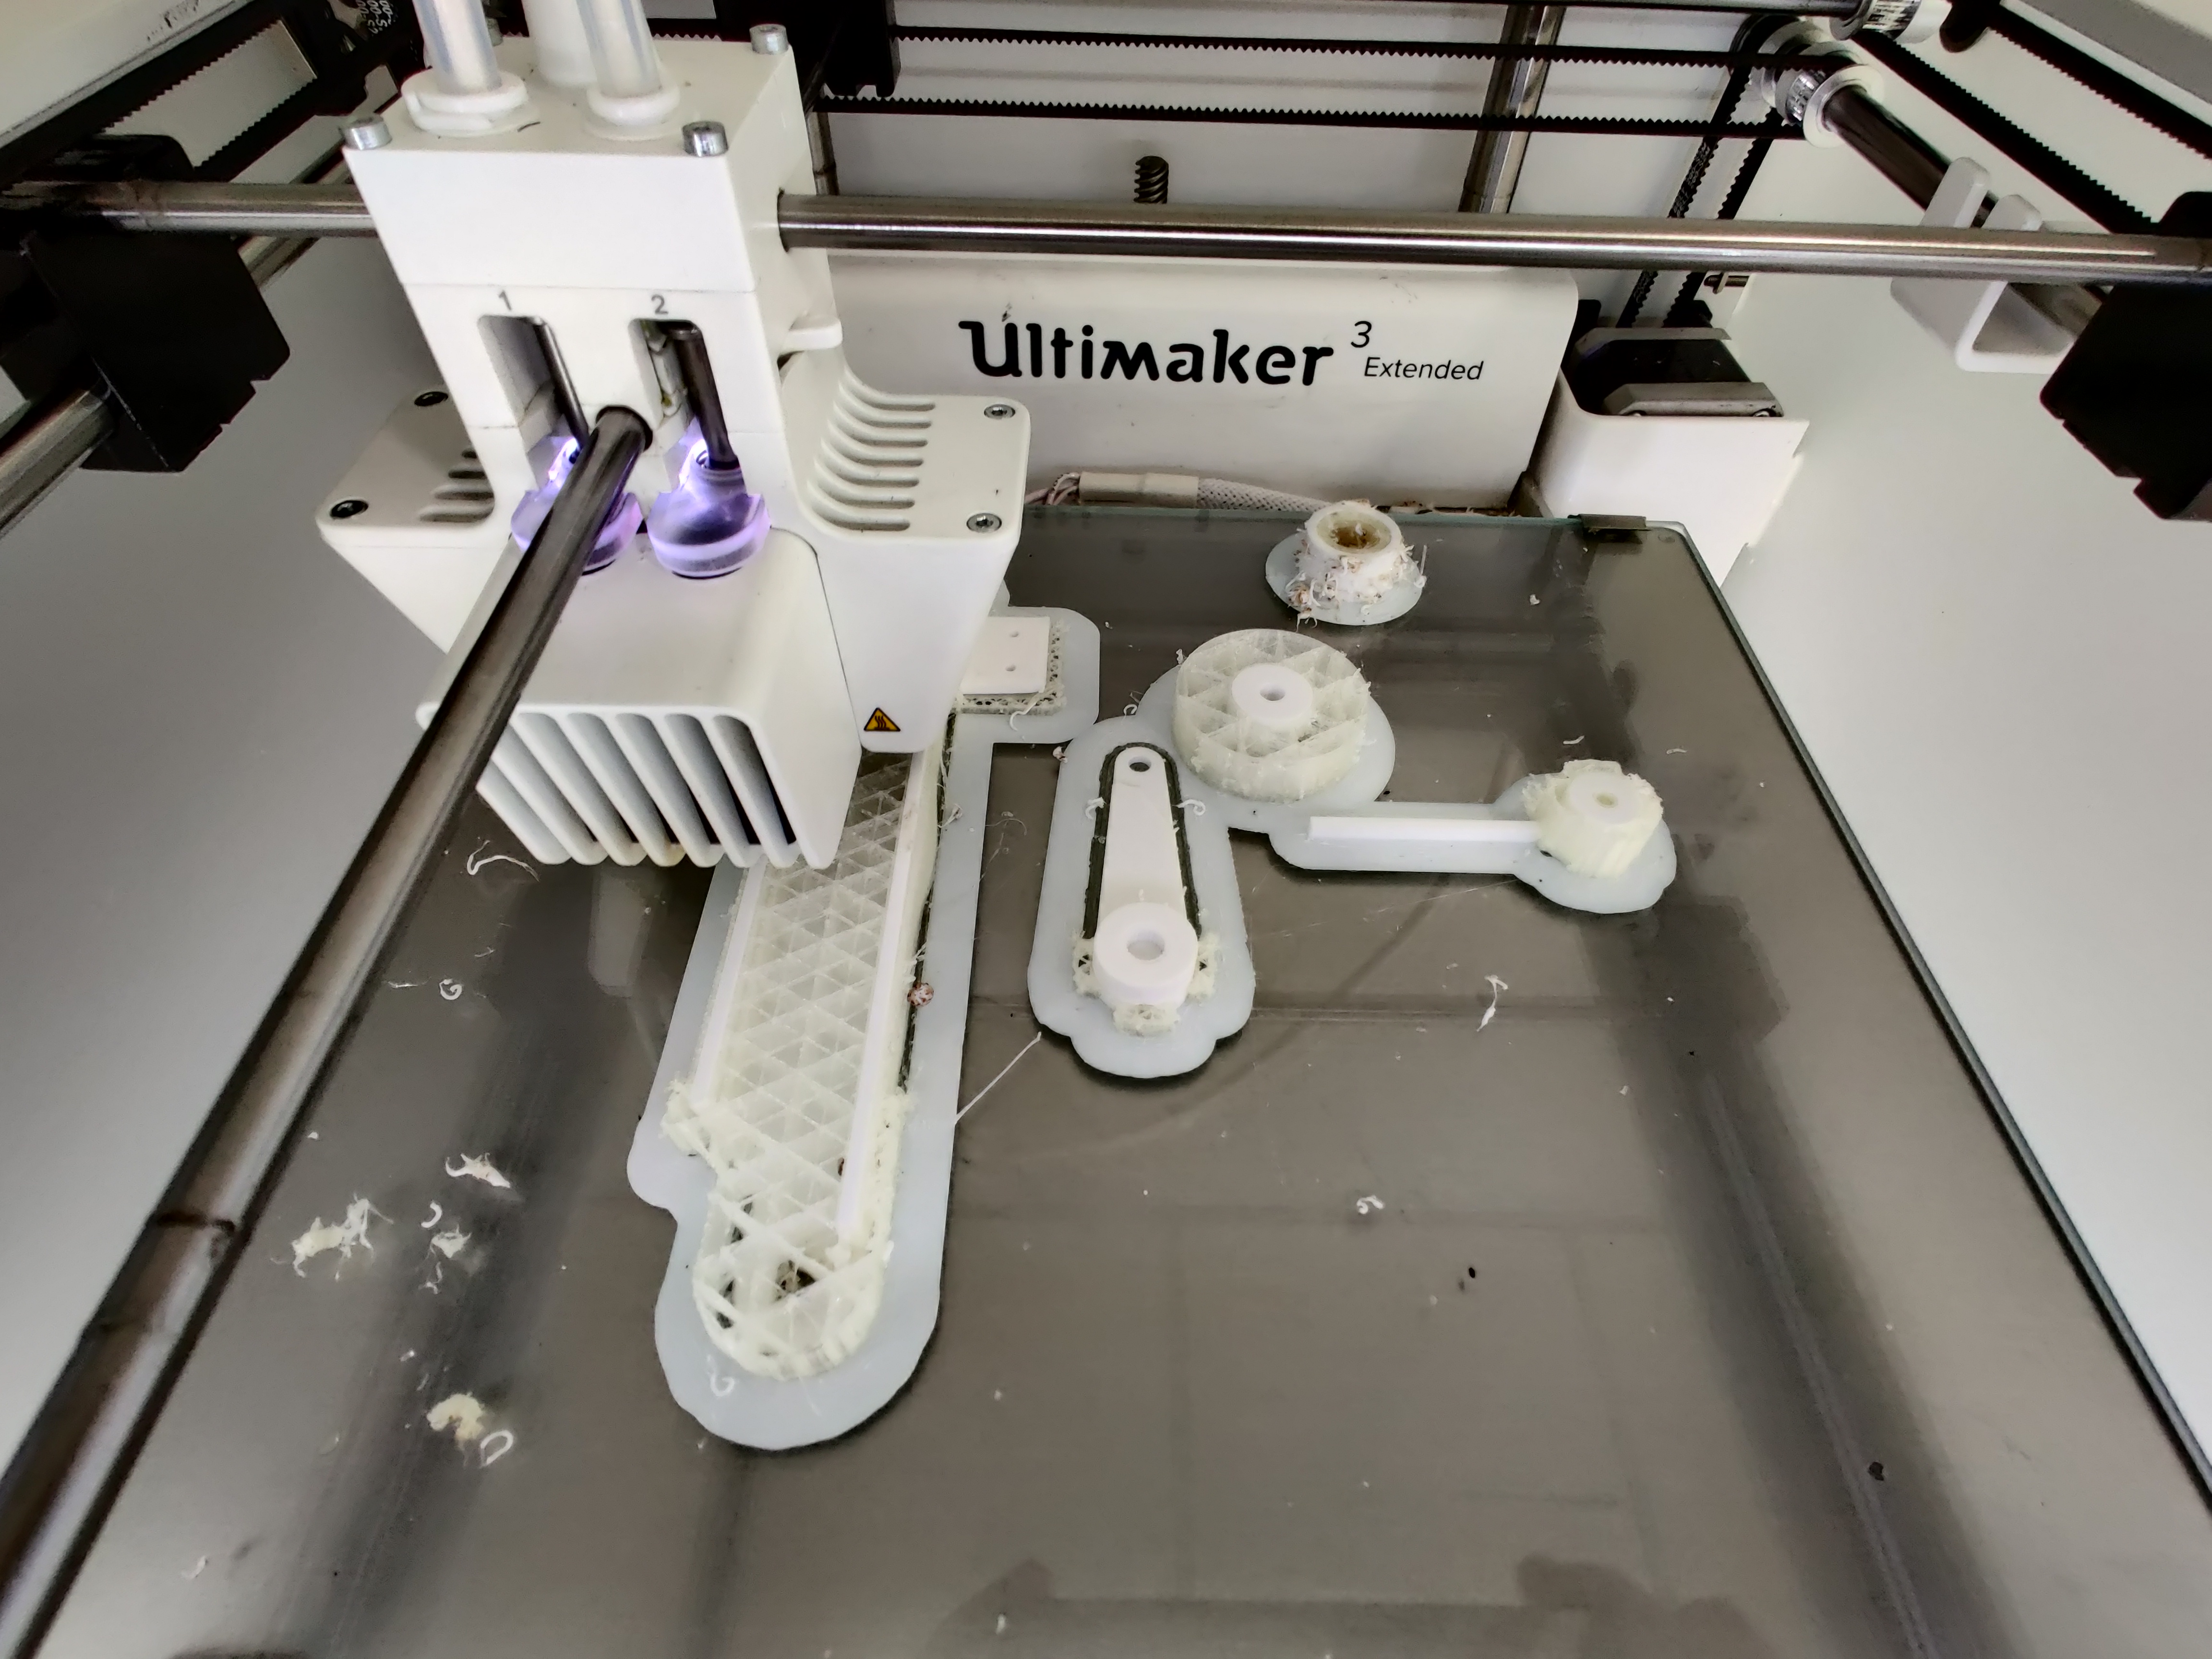
\includegraphics[width=\linewidth]{pictures/pieces_good.jpg}
    \end{minipage}
    \caption{Figuras siendo correctamente impresas tras reparar los extrusores y usando material nuevo.}
    \label{fig:good_pieces}
\end{figure}

\subsubsection*{Semana del 14 de septiembre}
Finalmente, pese a que se consiguió reparar parcialmente los cabezales de impresión, tras el
uso continuado, el extrusor del material de soporte de \ac{PVA} se acabó rompiendo por lo que
las impresiones tuvieron que detenerse. Por suerte, se contactó con unos alumnos
de la Escuela Técnica Superior de Telecomunicaciones y se pudo hacer un uso provisional
de sus impresoras 3D (ya que cuentan de un laboratorio de fabricación) para continuar el
desarrollo, usando además una Ultimaker 3, mismo modelo con el que se contaba en la
universidad (figura \ref{fig:telec}):

\begin{figure}[H]
    \centering
    \begin{minipage}{.49\linewidth}
        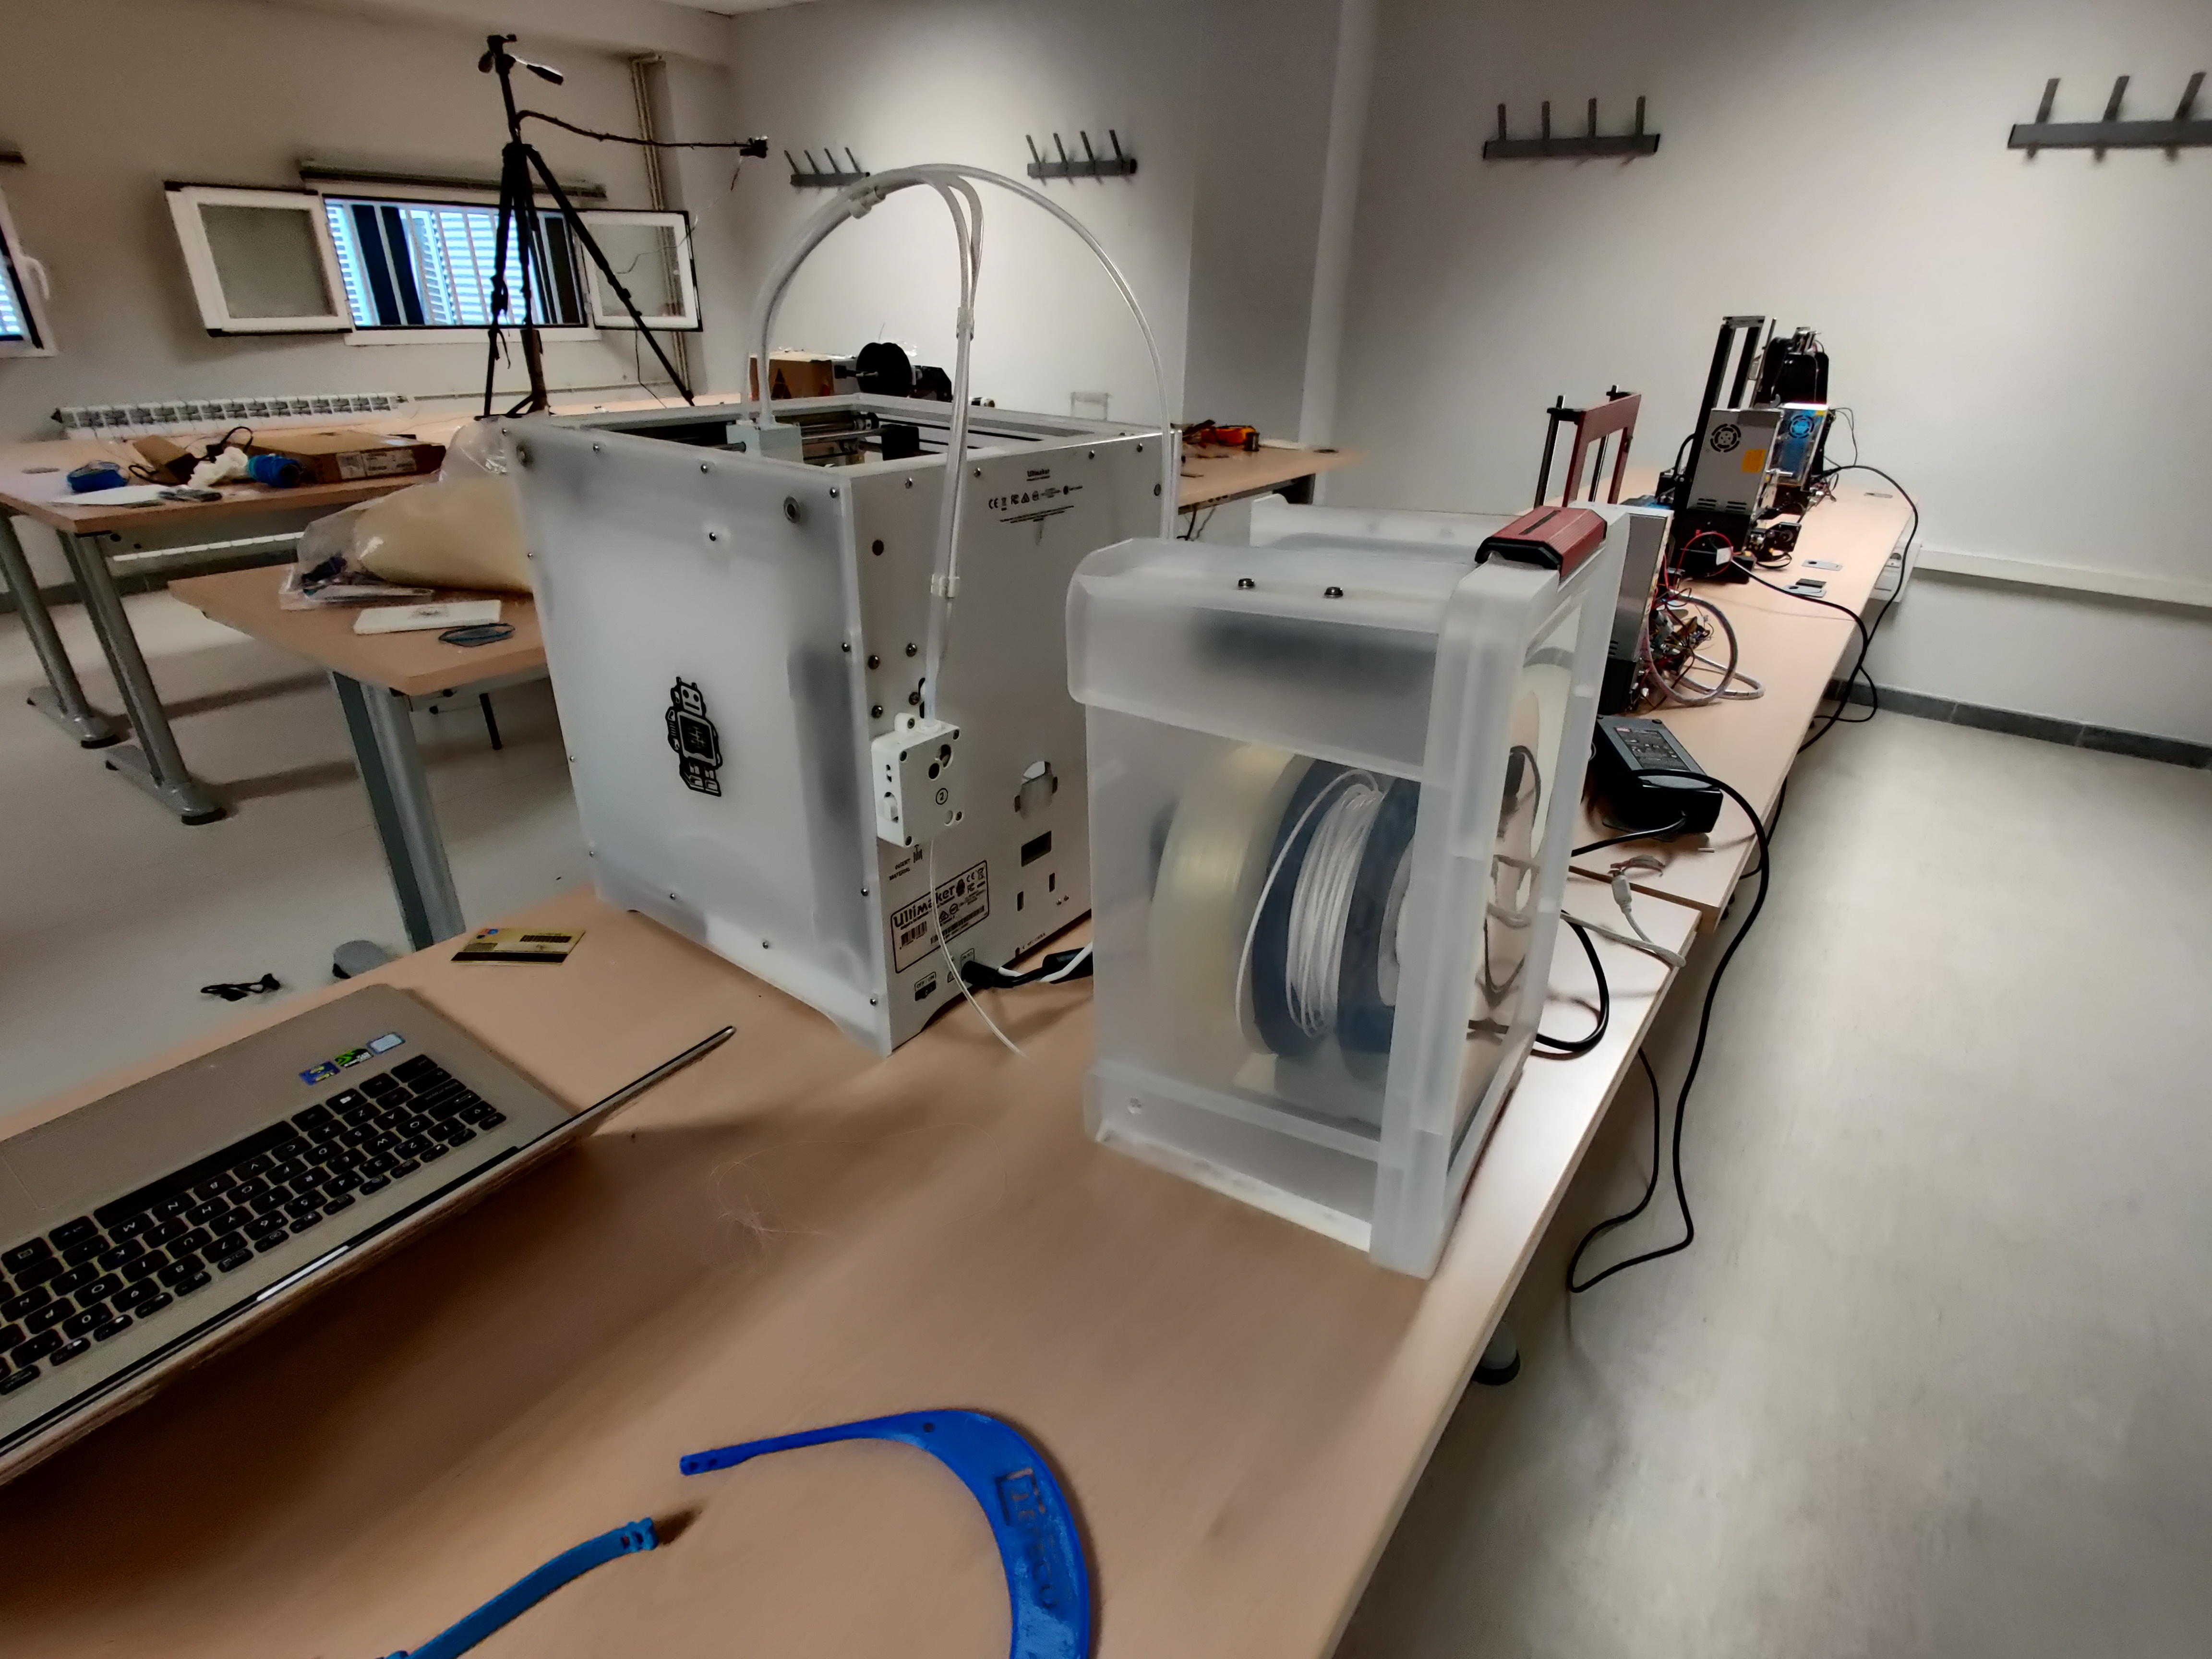
\includegraphics[width=\linewidth]{pictures/teleco-1.jpg}
    \end{minipage}
    \hfill
    \begin{minipage}{.49\linewidth}
        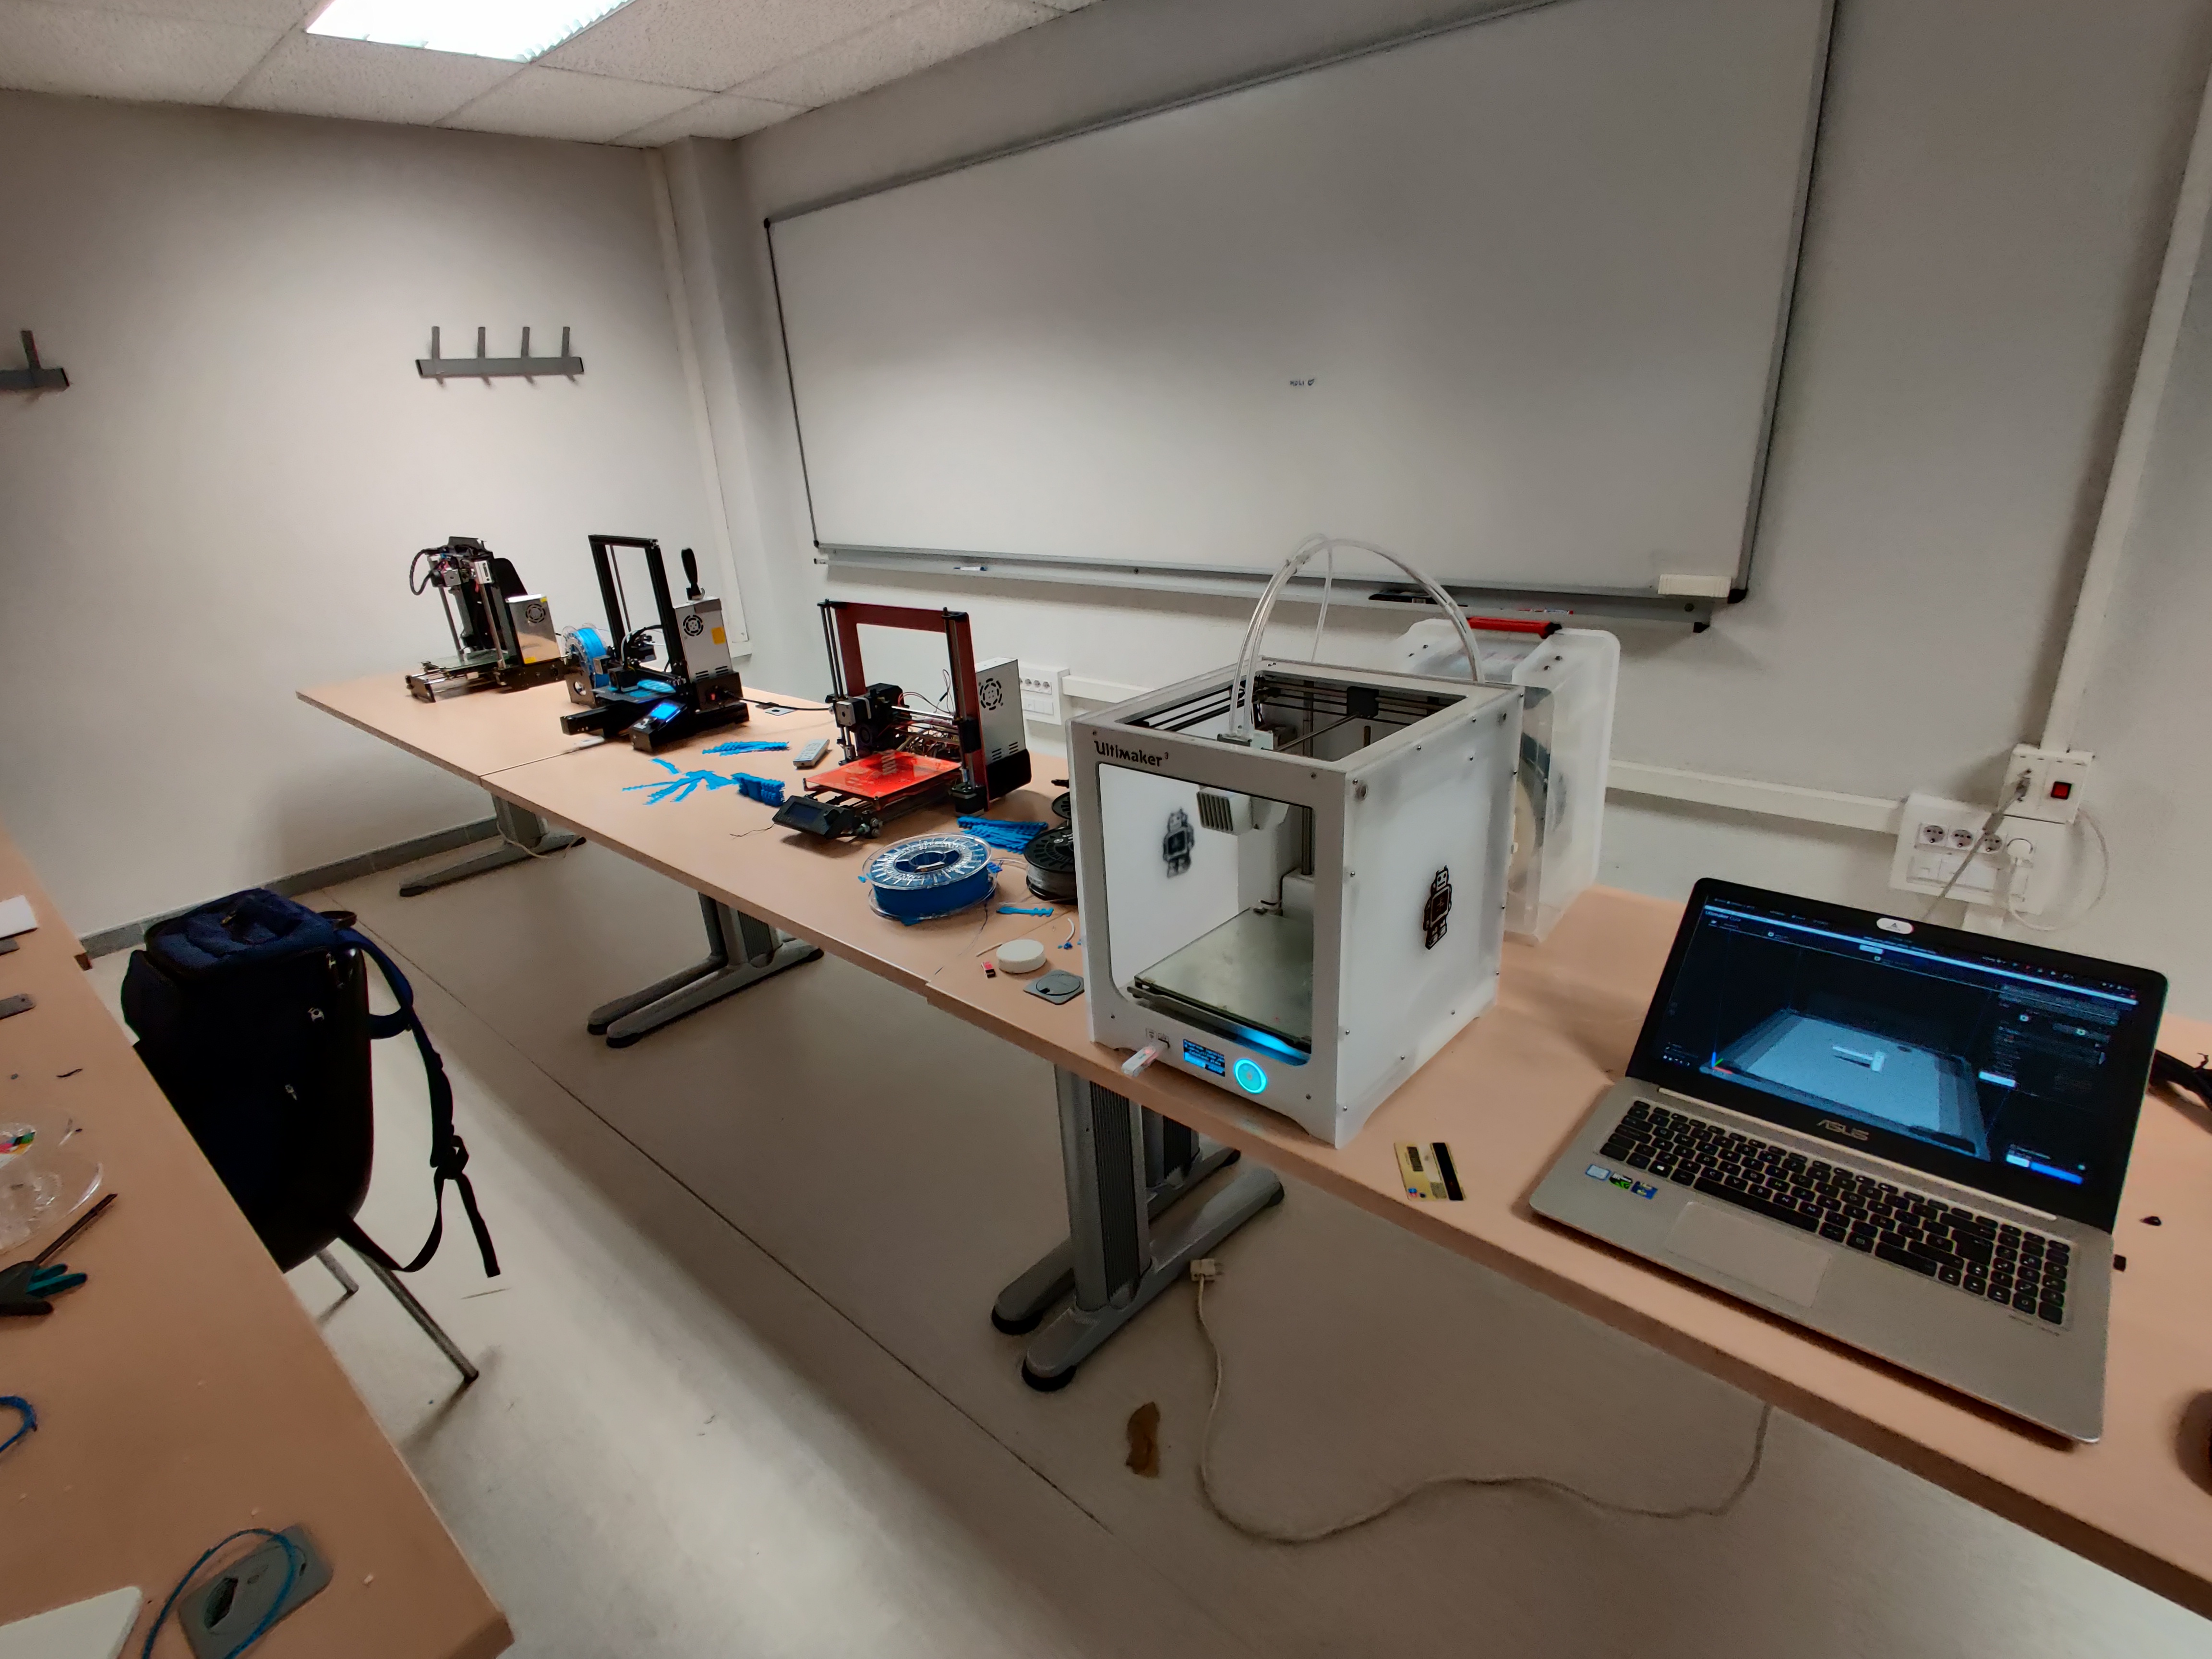
\includegraphics[width=\linewidth]{pictures/teleco_2.jpg}
    \end{minipage}
    \caption{Laboratorio de fabricación de la escuela de telecomunicaciones prestado temporalmente para continuar con el proyecto.}
    \label{fig:telec}
\end{figure}

Una vez se recibió el extrusor nuevo, se pudo continuar con las impresiones sin
más inconvenientes. Añadir que, después de cada impresión utilizando \ac{PVA}, era
necesario realizar un mantenimiento de los cabezales para evitar su obstrucción.